
\chapter{Desarrollo}
\label{cha:desarrollo}

\begin{FraseCelebre}
  \begin{Frase}
    Cada uno de nosotros debe trabajar para su propia mejora, y al mismo tiempo compartir una responsabilidad general para toda la humanidad.
  \end{Frase}
  \begin{Fuente}
    Marie Curie
  \end{Fuente}
\end{FraseCelebre}

\section{Introducción}
\label{sec:intro-desarrollo}

En el presente \gls{tfm} se ha desarrollado una estrategia de detección de objetos abandonados para ser aplicado en sistemas de videovigilancia. Como ya se comentó al final de la sección \ref{subsec:comparativa-detectores}, se utilizará como detector de objetos y personas \gls{yolov4} y como algoritmo de seguimiento \gls{deepsort}. A continuación, se describen las diferentes secciones que componen este capítulo.

Primero se evaluará \gls{yolov4} sobre Darknet, framework de código abierto escrito en C y \gls{cuda}, y se analizará la precisión y velocidad que se obtienen en la detección de objetos y personas. Posteriormente se convertirá el modelo de \gls{yolov4} de Darknet a Tensorflow, framework de código abierto escrito en Python y C++ orientado al desarrollo de algoritmos inteligentes de Machine Learning. Utilizar \gls{yolov4} con Tensorflow facilitará la programación del algoritmo de detección de objetos abandonados con Python, ya que Darknet no es un framework de uso extendido y podría ser más difícil encontrar soluciones para los posibles errores. A continuación se reentrenará el modelo de la red \gls{yolov4} sobre el dataset \gls{oidv4} para observar si se obtienen mayores valores en las métricas de calidad respecto a \gls{coco}.

Una vez obtenido el modelo de \gls{yolov4} definitivo, se probará el algoritmo de seguimiento \gls{deepsort}. Solo nos interesa la detección y seguimiento de personas y objetos de interés, por lo que se filtrará la detección para que solo se identifiquen las clases que queremos.

Finalmente, se expondrá una estrategia para la detección de objetos abandonados basada en la detección de objetos y personas mediante \gls{cnn}'s y se implementará sobre el detector de objetos \gls{yolov4} junto al algoritmo de detección \gls{deepsort}. En el planteamiento del algoritmo de detección de objetos abandonados se tendrá que considerar dos posibles escenarios. El primero es que se identifique un objeto sin propietario que se encuentre estacionario durante toda la ejecución de la secuencia de vídeo. En este caso, se emitirá una señal de alarma cuando se superen los 15 segundos del objeto inmóvil. En el segundo escenario se deberá de crear una asociación entre persona y objeto. Una vez establecida la asociación se podrá evaluar cuando una persona abandona un objeto de su propiedad a una una distancia en píxeles 5 veces mayor a la distancia a la que se encontraba en el momento que se realizó la asociación.

Cabe recalcar que en este capítulo se va a exponer cada uno de los procedimientos que se han llevado a cabo para poner en funcionamiento los algoritmos de detección, seguimiento y detección de objetos abandonados. Todos los resultados obtenidos durante el desarrollo de esta parte del proyecto se pueden consultar en el capítulo \ref{cha:resultados}.

\section{Detección de personas y objetos con YOLOv4}
\label{sec:desarrollo-yolov4}

Para la utilización de \gls{yolov4} se ha instalado previamente la librería opencv-python 4.1.1.26 junto con \gls{cuda} 10.1.243 y cuDNN 7.6.5 para poder codificar de manera más optima los algoritmos utilizando una \gls{gpu} NVIDIA.

Se ha clonado el repositorio de \gls{yolov4} de GitHub \cite{yolov4-darknet-github} en el framework Darknet. Para obtener el máximo rendimiento por parte del equipo que se está utilizando se ha modificado el fichero Makefile para habilitar la utilización de la \gls{gpu} junto con \gls{cuda}, así como OpenCV para poder visualizar por pantalla los resultados las de las detecciones.

En la evaluación del algoritmo de detección de \gls{yolov4} se va a emplear una \gls{gpu} NVIDIA Tesla T4 del servicio cloud de Google Colab \cite{google-colab}, un servicio cloud de Google basado en los Notebooks de Jupyter donde ya vienen instaladas la mayoría de librerías necesarias para la programación de algoritmos de Machine Learning. Esta \gls{gpu} tiene una capacidad de computación de 7,5 por lo que será necesario descomentar una línea del fichero Makefile para indicar que se está empleando una \gls{gpu} con esas características. Tras modificar el fichero se ha ejecutado el comando make para compilar el repositorio, de tal manera que se generan los ficheros necesarios para el funcionamiento de la red neuronal de \gls{yolov4} sobre Darknet. 

\vspace{0.5cm}
\begin{lstlisting}[language=iPython,caption=Evaluación del detector de objetos YOLOv4 en Darknet (1),captionpos=b,label={lst:evaluate-yolov4-darknet1}]
# Clonar el repositorio de GitHub de YOLOv4 darknet
git clone https://github.com/AlexeyAB/darknet

# Entrar dentro de la carpeta del repositorio
cd darknet

# Modificar las siguientes lineas del fichero makefile para habilitar la GPU y OPENCV
sed -i 's/OPENCV=0/OPENCV=1/' Makefile
sed -i 's/GPU=0/GPU=1/' Makefile
sed -i 's/CUDNN=0/CUDNN=1/' Makefile
sed -i 's/CUDNN_HALF=0/CUDNN_HALF=1/' Makefile
sed -i 's/# ARCH= -gencode arch=compute_75/ARCH= -gencode arch=compute_75/' Makefile

# Compilar mediante el comando make
make
\end{lstlisting}

Otro fichero que es necesario de modificar antes de ejecutar el algoritmo de detección es el fichero yolov4.cfg que es encuentra dentro de la carpeta \texttt{./cfg}. Este fichero contiene parámetros de configuración de la \gls{cnn} de \gls{yolov4} como el learning rate, max batches, momentum o hue, necesarios para el entrenamiento de la red, las dimensiones de las imágenes que se introducen a la capa de entrada de la red o los filtros y clases que se deben de tener en cuenta tanto para el entrenamiento como para la evaluación.

Se ha modificado los parámetros de \texttt{batch} y \texttt{subdivisions} con un valor de 1, ya que se va a usar la red para testear y no para entrenarla. Estos parámetros determinan la cantidad de imágenes que son procesadas de manera paralela.

\vspace{0.5cm}
\begin{lstlisting}[language=iPython,caption=Evaluación del detector de objetos YOLOv4 en Darknet (2),captionpos=b,label={lst:evaluate-yolov4-darknet2}]
# Cambiar batch y subdivisions de yolov4.cfg para test
cd cfg
sed -i 's/batch=64/batch=1/' yolov4.cfg
sed -i 's/subdivisions=8/subdivisions=1/' yolov4.cfg
cd ..

# Descargar los pesos preentrenados de YOLOv4
wget https://github.com/AlexeyAB/darknet/releases/download/darknet_yolo_v3_optimal/yolov4.weights

# Ejecutar detector de objetos en video con YOLOv4 en Darknet
./darknet detector demo cfg/coco.data cfg/yolov4.cfg yolov4.weights ./data/videos-datasets/{input_file_name.avi} -i 0 -out_filename ./results/{output_file_name.avi}
\end{lstlisting}

Se han descargado los pesos de \gls{yolov4} previamente entrenados sobre el dataset \gls{coco}. Por último se ha ejecutado el algoritmo de detección de objetos. En el código \ref{lst:evaluate-yolov4-darknet3} se especifica que la detección es en formato vídeo, se va a utilizar \gls{yolov4} como detector y la ubicación tanto del vídeo de entrada que se quiere procesar como el vídeo de salida resultante de las detecciones.

\vspace{0.5cm}
\begin{lstlisting}[language=iPython,caption=Evaluación del detector de objetos YOLOv4 en Darknet (3),captionpos=b,label={lst:evaluate-yolov4-darknet3}]
# Descargar los pesos preentrenados de YOLOv4
wget https://github.com/AlexeyAB/darknet/releases/download/darknet_yolo_v3_optimal/yolov4.weights

# Ejecutar detector de objetos en video con YOLOv4 en Darknet
./darknet detector demo cfg/coco.data cfg/yolov4.cfg yolov4.weights ./data/videos-datasets/{input_file_name.mp4} -i 0 -out_filename ./results/{output_file_name.avi}
\end{lstlisting}

En la figura \ref{fig:detection-yolov4-darknet-pets2007} se muestra el funcionamiento de \gls{yolov4} en Darknet donde se puede observar un escenario lleno de personas y equipajes como bolsas de mano, mochilas y maletas.

\begin{figure}[ht]
\centering
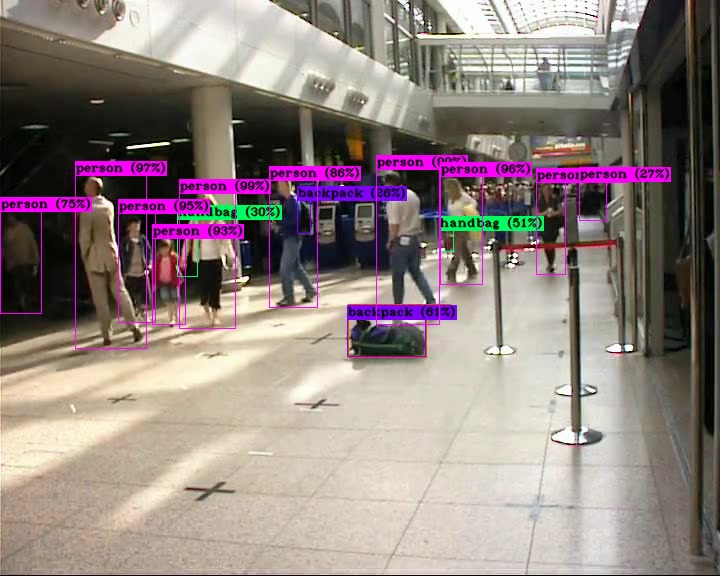
\includegraphics[width=0.4\textwidth]{img/chapters/desarrollo/S08-fourthView-detection.jpg}
\caption{\label{fig:detection-yolov4-darknet-pets2007}Detección de objetos con YOLOv4 en Darknet en \cite{pets2007-dataset}}
\end{figure}

Las últimas evaluaciones del algoritmo de detección de \gls{yolov4} en Darknet se han realizado con Google Colab. En el siguiente \href{https://colab.research.google.com/drive/1kXcZL7iZ2sZmyFuQ6GwVFfkfyha6A6nr?usp=sharing}{link} se puede ejecutar el Notebook de Google Colab donde se realizan los mismos pasos descritos anteriormente.

Durante el desarrollo del proyecto se ha decidido convertir el modelo de Darknet a Tensorflow, ya que se trata de un framework que emplea Python y facilitará la tarea de diseño del algoritmo de detección de objetos al no basarse únicamente en Darknet, framework que no es de uso extendido y puede ser una tarea complicada su utilización cuando aparezcan posibles errores.

Para la utilización de \gls{yolov4} basado en Tensorflow se necesita convertir el modelo. La implementación que se expone a continuación está totalmente inspirada en \cite{yolov4-tf-github-original}. A continuación, se describen los pasos que se han seguido para poner en funcionamiento de \gls{yolov4} sobre Tensorflow 2.3.0rc0.

Primero se ha clonado el repositorio \cite{yolov4-tf-github}, el cual es un \textit{fork} de \cite{yolov4-tf-github-original}, y se han instalado las librerías y dependencias necesarias que se contemplan en el fichero \texttt{requirements-gpu.txt}. Para facilitar su instalación se ha creado con Anaconda un entorno virtual. La instalación de Anaconda y el entorno virtual se explica con mayor detalle en la sección \ref{subsec:instalacion-anaconda} y en la sección \ref{subsec:creacion-entorno}.

\vspace{0.5cm}
\begin{lstlisting}[language=iPython,caption=Evaluación del detector de objetos YOLOv4 en Tensorflow (1),captionpos=b,label={lst:evaluate-yolov4-tf1}]
# Descarga del repositorio de GitHub
git clone https://github.com/jmudy/tensorflow-yolov4-tflite

# Entrar dentro de la carpeta del repositorio
cd tensorflow-yolov4-tflite

# Descarga de los pesos de YOLOv4
wget https://github.com/AlexeyAB/darknet/releases/download/darknet_yolo_v3_optimal/yolov4.weights -P ./data/

# Crear entorno de Anaconda basado en Python 3.7.0 y acceder a el
conda env create -f conda-gpu.yml
conda activate yolov4-gpu
\end{lstlisting}

En el código \ref{lst:evaluate-yolov4-tf2} se muestra el comando para convertir el modelo preentrenado de \gls{yolov4} en Darknet a Tensorflow. Se ha especificado un tamaño de 608x608, por dos motivos. El primero, es el mismo tamaño de redimensionamiento de las imágenes a la entrada de la capa de la red que en Darknet, con lo cual, se puede comparar ambos modelos en las mismas condiciones. Segundo, se han obtenido mejores resultados que empleando el clásico tamaño de 416x416.

\vspace{0.5cm}
\begin{lstlisting}[language=iPython,caption=Evaluación del detector de objetos YOLOv4 en Tensorflow (2),captionpos=b,label={lst:evaluate-yolov4-tf2}]
# Convertir pesos de YOLOv4 Darknet a Tensorflow
python save_model.py --weights ./data/yolov4.weights --output ./checkpoints/yolov4-608 --input_size 608 --model yolov4
\end{lstlisting}

En el código \ref{lst:evaluate-yolov4-tf3} se puede apreciar el comando que se ha utilizado para la ejecución del algoritmo de detección de objetos en \gls{yolov4} en Tensorflow. Como se puede observar en las primeras líneas del script \texttt{detect\_video.py} \cite{yolov4-tf-github-original}, se disponen de una serie de flags donde se pueden indicar una gran variedad de parámetros. En este caso, se ha indicado que se quiere utilizar un modelo de \gls{yolov4} convertido con tamaño de redimensionamiento 608x608 (si no se indica, el código por defecto busca un modelo de tamaño 416x416). También se ha especificado que se quiere emplear como detector \gls{yolov4}, ya que este repositorio también permite ejecutar la detección de objetos sobre \gls{yolo}v3. Del mismo modo que con Darknet, en el siguiente \href{https://colab.research.google.com/drive/1ZwcfV2hFZKcsyXaqKp9AGuEi5TY-QwVW?usp=sharing}{link} se puede consultar el Notebook de Google Colab donde se realizan los mismos pasos descritos anteriormente.

\vspace{0.5cm}
\begin{lstlisting}[language=iPython,caption=Evaluación del detector de objetos YOLOv4 en Tensorflow (3),captionpos=b,label={lst:evaluate-yolov4-tf3}]
# Ejecutar algoritmo de deteccion de objetos YOLOv4 en Tensorflow
!python detect_video.py --weights ./checkpoints/yolov4-608 --size 608 --model yolov4 --video {input_file_name.mp4} --output {output_file_name.avi}
\end{lstlisting}

En la figura \ref{fig:detection-yolov4-darknet-gba-far-video3} se muestra un ejemplo del funcionamiento de \gls{yolov4} en Tensorflow donde se puede observar el hall de una Universidad llena de personas y equipajes como bolsas de mano y maletas.

\begin{figure}[ht]
\centering
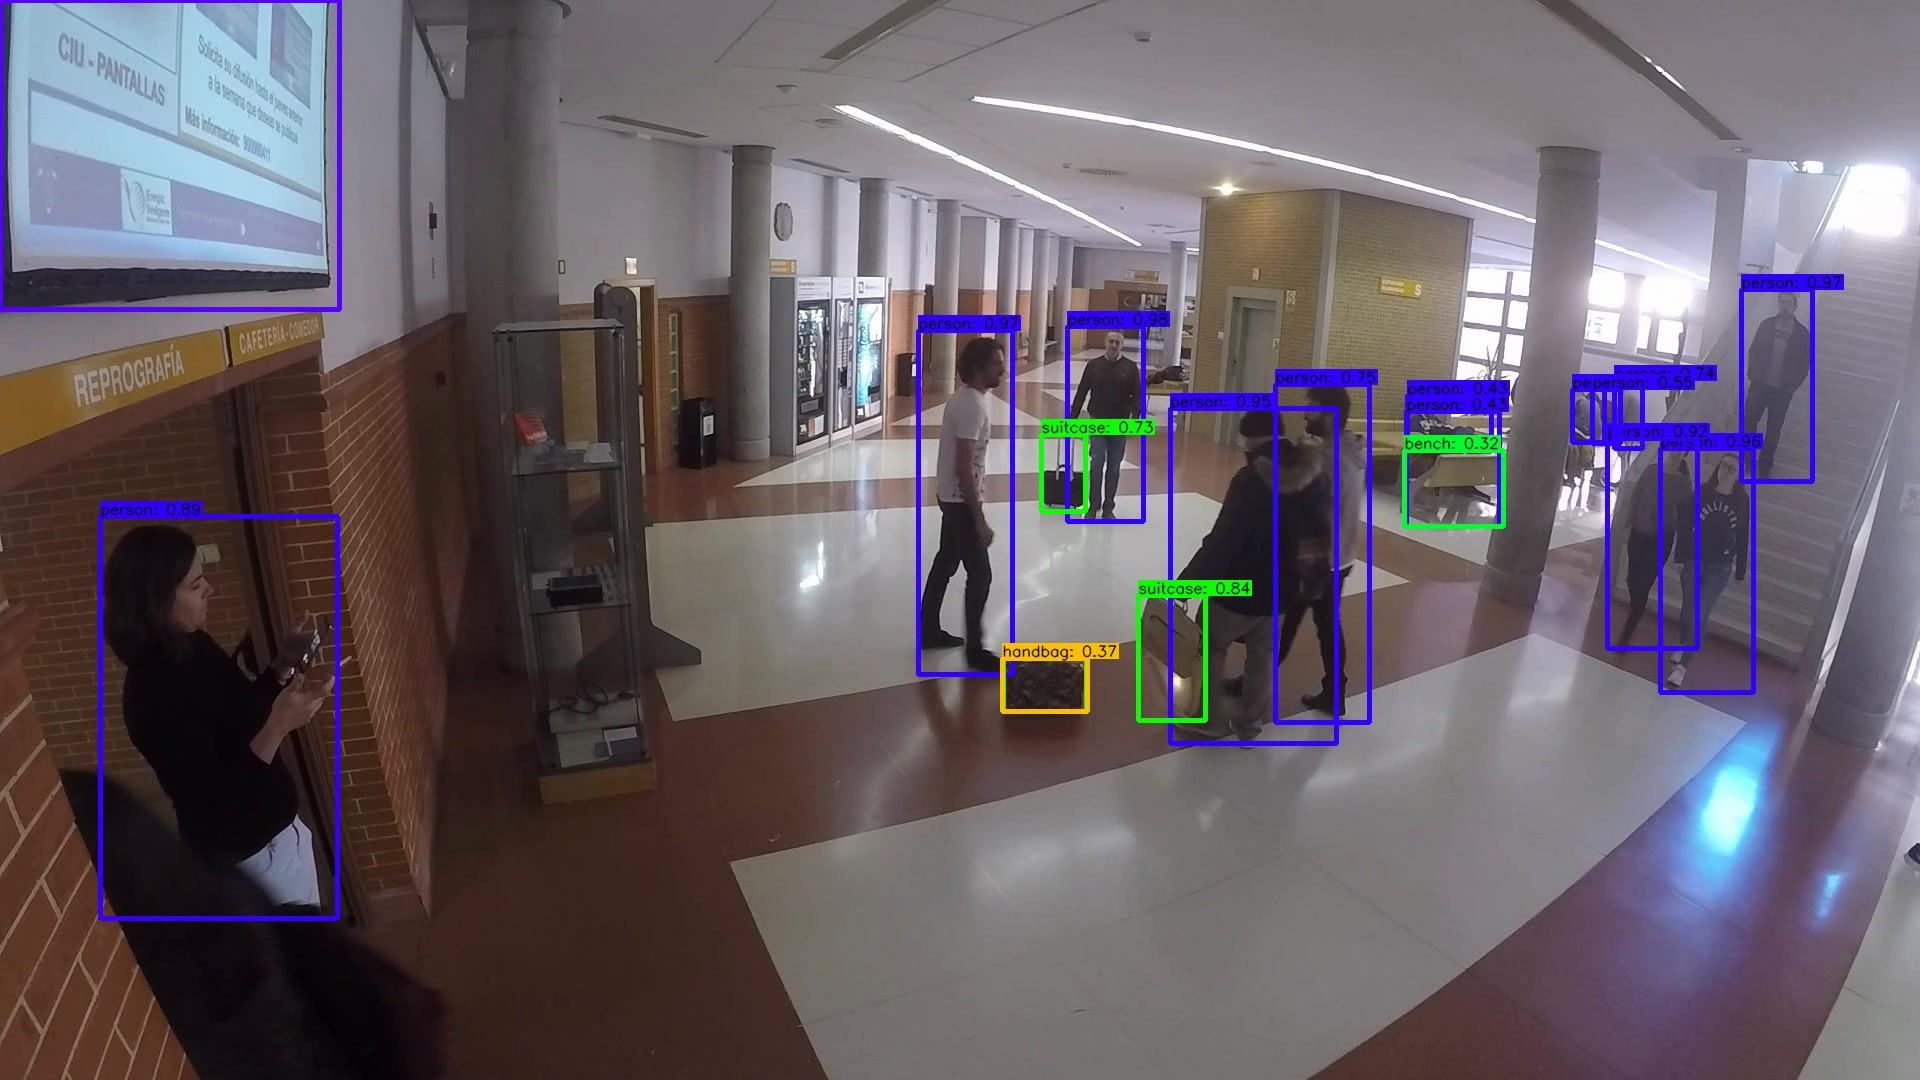
\includegraphics[width=0.45\textwidth]{img/chapters/desarrollo/GBA-far-video3-detection.jpg}
\caption{\label{fig:detection-yolov4-darknet-gba-far-video3}Detección de objetos con YOLOv4 en Tensorflow en \cite{gba-dataset}}
\end{figure}

Como se puede observar en la figura \ref{fig:predictions-darknet-tf} se puede apreciar que la precisión en las detecciones de \gls{yolov4} en Darknet y Tensorflow son prácticamente idénticas. Por tanto, se continuará el desarrollo del proyecto empleando Tensorflow como framework para la evaluación y diseño de los distintos algoritmos utilizados. En la sección \ref{subsec:resultados-yolov4-tf} se analizará con detalle las detecciones de objetos de \gls{yolov4} en Tensorflow.

\begin{figure}[ht]
  \centering
  \begin{subfigure}[b]{0.35\textwidth}
    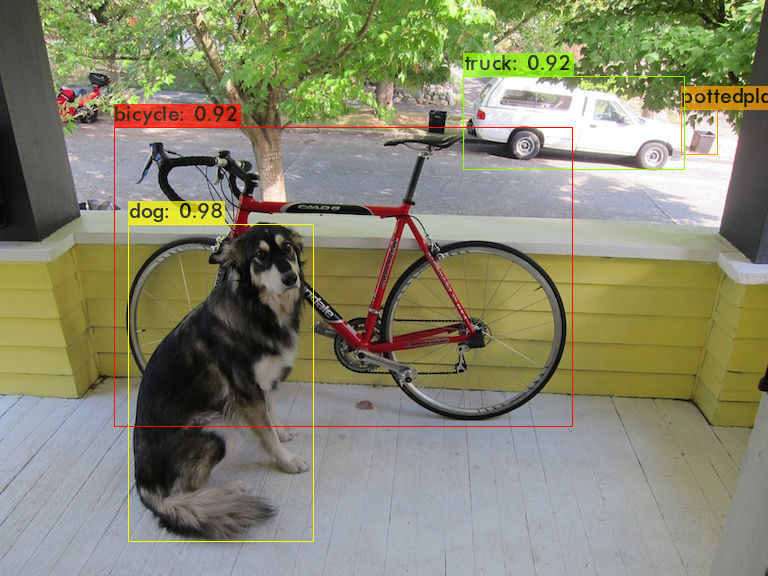
\includegraphics[width=\textwidth]{img/chapters/desarrollo/predictions.jpg}
    \caption{}
    \label{fig:predictions-darknet}
  \end{subfigure}
  \qquad\qquad
  \begin{subfigure}[b]{0.35\textwidth}
    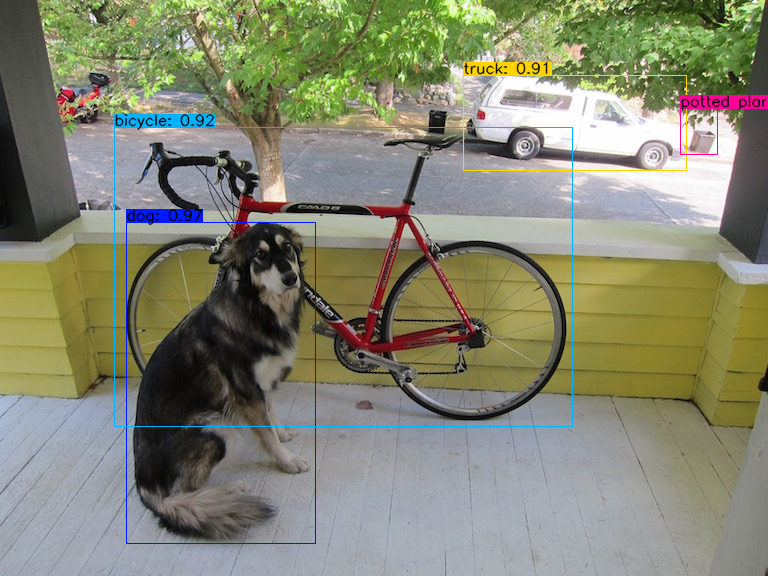
\includegraphics[width=\textwidth]{img/chapters/desarrollo/detection1.png}
    \caption{}
    \label{fig:predictions-tf}
  \end{subfigure}
  \caption{Detecciones de YOLOv4 con Darknet y Tensorflow.
    (\protect\subref{fig:predictions-darknet}) Detección de YOLOv4 con Darknet.
    (\protect\subref{fig:predictions-tf}) Detección de YOLOv4 con Tensorflow.}
  \label{fig:predictions-darknet-tf}
\end{figure}

\section{Datasets utilizados para el evaluación de YOLOv4}
\label{sec:datasets-utilizados}

La detección de objetos con \gls{yolov4} está basada en \gls{coco}, un dataset que contiene 80 categorías de objetos muy diversos y que se adaptan excelentemente a la problemática que se presenta en este proyecto. Contiene imágenes de las clases de interés: personas, mochilas, bolsos y maletas.

Para poder contrastar los resultados obtenidos en la evaluación de las métricas de calidad de \gls{coco} sobre \gls{yolov4}, se va a emplear el dataset \gls{oidv4}, donde previamente se entrenará un modelo de detección en base a las imágenes de \gls{oidv4}. La ventaja de utilizar \gls{oidv4} es que dispone de 600 categorías de objetos para evaluar los algoritmos de detección de objetos. De esta manera, se puede construir un gran dataset más específico y además con más clases de interés que las que ofrece \gls{coco}.

En las siguientes secciones se explicará en mayor profundidad y detalle como están formados los datasets \gls{coco} y \gls{oidv4}.

\subsection{MS COCO Dataset}
\label{subsec:coco-dataset}

El dataset \gls{coco} \cite{lin2015microsoft} es un conjunto de datos de referencia utilizado para evaluar el rendimiento de los modelos entrenados por visión por computadora. Está diseñado para representar una amplia gama de objetos que encontramos regularmente en la vida cotidiana (ver figura \ref{fig:cocodataset}).

\begin{figure}[ht]
\centering
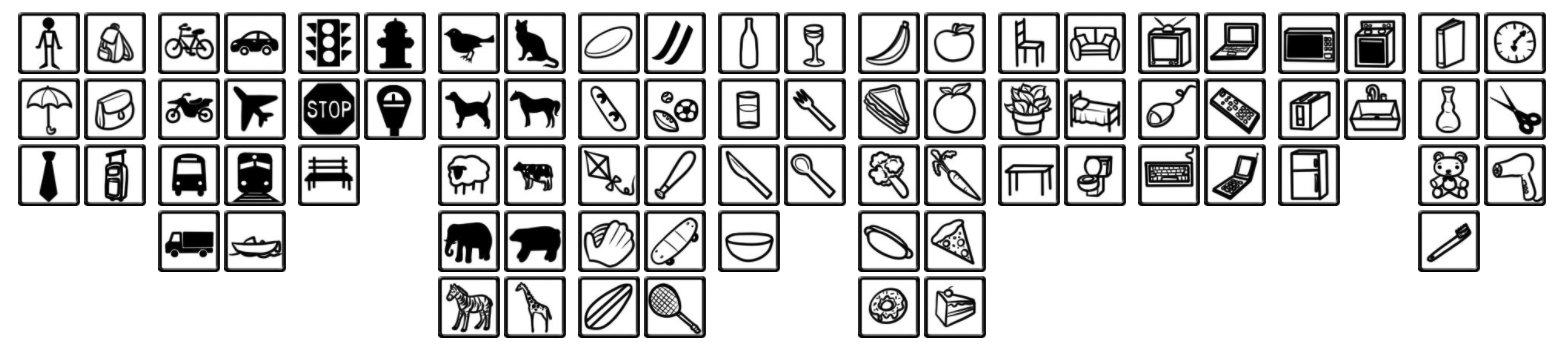
\includegraphics[width=0.9\textwidth]{img/chapters/desarrollo/cocodataset.png}
\caption{\label{fig:cocodataset}Categorías de objetos del dataset MS COCO \cite{coco-official-website}}
\end{figure}

\gls{coco} está etiquetado en un formato especial llamado COCO JSON, y proporciona datos para entrenar modelos supervisados de visión por computadora que son capaces de identificar los objetos comunes del conjunto de datos. Estos modelos están lejos de ser perfectos, por lo que el dataset \gls{coco} proporciona un punto de referencia para evaluar la mejora periódica de estos modelos a través de la investigación en visión por computadora.

Otra motivación para el dataset \gls{coco} es proporcionar un conjunto de datos base para entrenar modelos de visión por computadora. Una vez entrenado el modelo, se puede perfeccionar para aprender otras tareas, como las que se van a describir a continuación.

\subsubsection*{Tareas de MS COCO}
\label{subsubsec:tareas-coco}

\gls{coco} tiene múltiples tareas de visión por computadora. A continuación, se enumeran en orden decreciente en base a su uso:

\begin{itemize}
    \item \textbf{Detección de objetos}: los objetos se anotan con un cuadro delimitador y una etiqueta de clase. El dataset \gls{coco} tiene 121.408 imágenes para detección de objetos, 883.331 anotaciones de objetos, 80 clases y una resolución media de imagen de 640x480.
    
    \begin{figure}[ht]
    \centering
    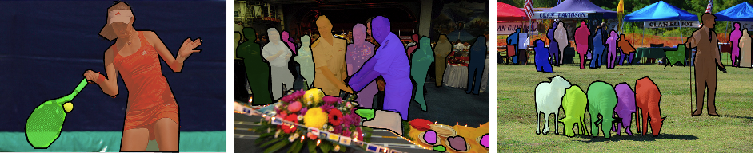
\includegraphics[width=0.65\textwidth]{img/chapters/desarrollo/detection-splash.png}
    \caption{\label{fig:detection-splash}MS COCO detección de objetos \cite{coco-official-website}}
    \end{figure}
    
    \item \textbf{Segmentación semántica}: los límites de los objetos se etiquetan con una máscara y las clases de objetos se etiquetan con una etiqueta de clase. La segmentación semántica requiere modelos para trazar los límites entre los objetos.
    
    \begin{figure}[ht]
    \centering
    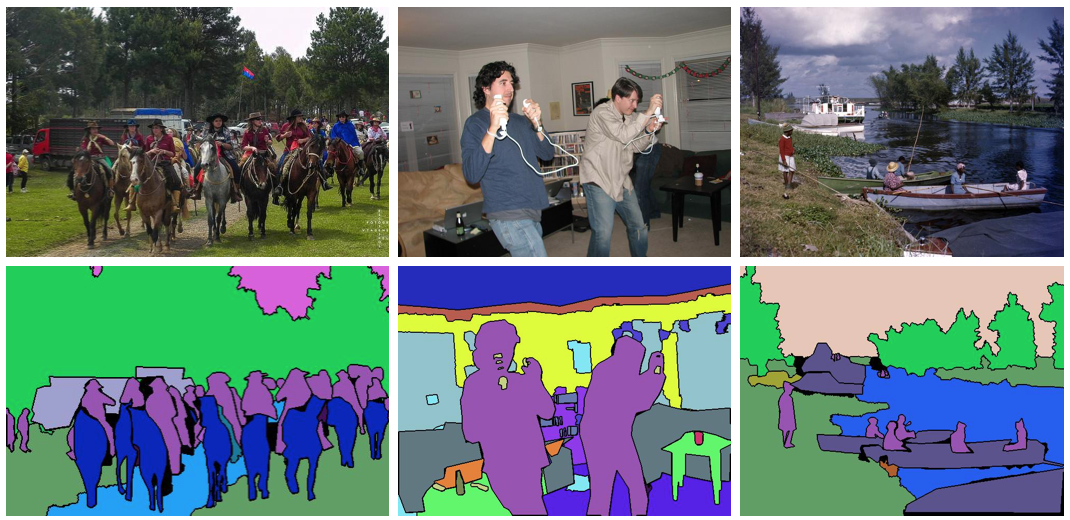
\includegraphics[width=0.6\textwidth]{img/chapters/desarrollo/panoptic-splash.png}
    \caption{\label{fig:panoptic-splash}MS COCO segmentación semántica \cite{coco-official-website}}
    \end{figure}    
    
    \item \textbf{Detección de puntos clave}: las personas son etiquetadas con puntos claves de interés (como pueden ser codos, rodillas o cabezas). El dataset \gls{coco} dispone de 250.000 personas con puntos clave etiquetados.
    
    \begin{figure}[ht]
    \centering
    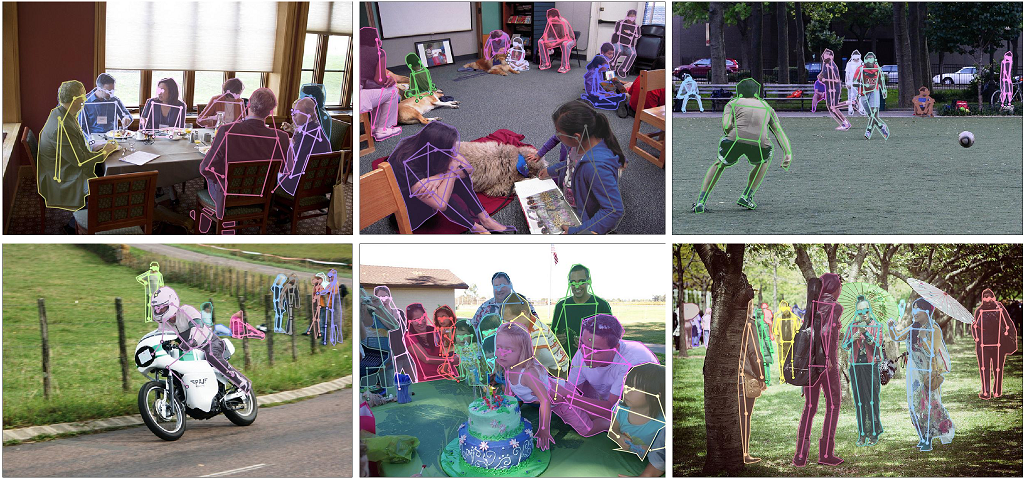
\includegraphics[width=0.6\textwidth]{img/chapters/desarrollo/keypoints-splash-big.png}
    \caption{\label{fig:keypoints-splash-big}MS COCO detección de puntos clave \cite{coco-official-website}}
    \end{figure}    
    
\end{itemize}

\subsection{Open Images Dataset v4}
\label{subsec:OIDv4-dataset}

\gls{oidv4} \cite{Kuznetsova_2020} es un conjunto de datos de 9,2 millones de imágenes con anotaciones en formato .txt unificadas para la clasificación de imágenes, detección de objetos y detección de relaciones visuales (ver figura \ref{fig:example-annotations-oidv4}). Las imágenes tienen una licencia Creative Commons Attribution que permite compartir y adaptar el material descargado de Flickr sin una lista predefinida de nombres de clases o etiquetas.

\begin{figure}[ht]
\centering
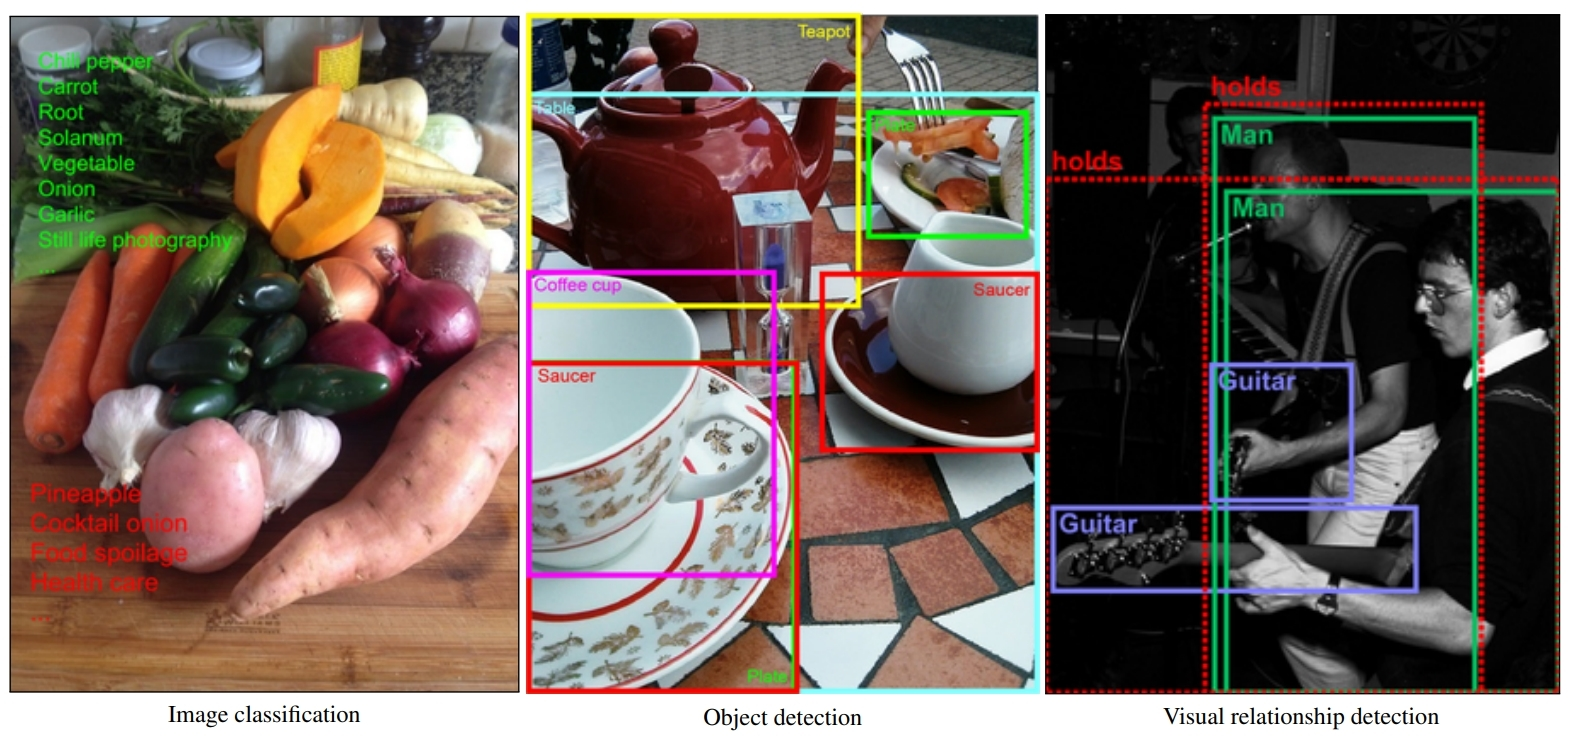
\includegraphics[width=0.6\textwidth]{img/chapters/desarrollo/example-annotations-oidv4.jpg}
\caption{\label{fig:example-annotations-oidv4}Ejemplo anotaciones en Open Images Dataset v4 \cite{Kuznetsova_2020}}
\end{figure}

\gls{oidv4} ofrece una gran escala en varias dimensiones: 30,1 millones de etiquetas a nivel de imagen para 19,8 mil conceptos, 15,4 millones de cuadros delimitadores para las 600 clases de objetos que se muestran en la figura \ref{fig:oidv4dataset}, y 375 mil anotaciones de relaciones visuales que involucra a 57 clases. Para la detección de objetos se proporciona más de 15 veces cuadros delimitadores que otros grandes datasets como \gls{coco} o ImageNet. Las imágenes suelen mostrar escenas complejas con varios objetos (de promedio tiene 8 objetos anotados por imagen). 

\begin{figure}[ht]
\centering
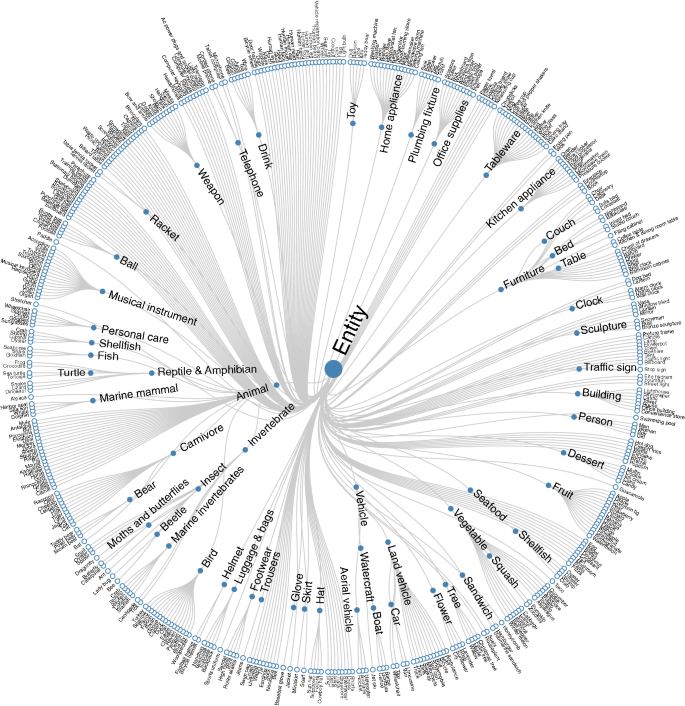
\includegraphics[width=0.65\textwidth]{img/chapters/desarrollo/oidv4-classes.png}
\caption{\label{fig:oidv4dataset}Categorías de objetos del dataset Open Images Dataset v4 \cite{Kuznetsova_2020}}
\end{figure}

\section{Evaluación de las métricas de calidad de MS COCO dataset}
\label{sec:evaluate-cocodataset}

En está sección se va a realizar la evaluación de las métricas de calidad del dataset \gls{coco} para tener una referencia a la hora de valorar, si reentrenando la red, se pueden obtener mejores métricas para la aplicación del proyecto.

Primero se ha descargado el repositorio oficial de \gls{yolov4} de GitHub \cite{yolov4-darknet-github}. Para aprovechar maximizar la eficiencia de la evaluación se ha modificado el fichero Makefile para habilitar la \gls{gpu} junto con \gls{cuda} y OpenCV. En esta evaluación se ha utilizado una NVIDIA Tesla T4, por lo que también ha sido necesario especificar que se va a utilizar una \gls{gpu} con una capacidad de cálculo de 7,5.

\vspace{0.5cm}
\begin{lstlisting}[language=iPython,caption=Evaluación de las métricas de calidad de MS COCO en YOLOv4 Darknet (1),captionpos=b,label={lst:evaluate-cocodataset1}]
# Clonar el repositorio de GitHub de YOLOv4 darknet
git clone https://github.com/AlexeyAB/darknet

# Entrar dentro de la carpeta del repositorio
cd darknet

# Modificar las siguientes lineas del fichero makefile para habilitar la GPU y OPENCV
sed -i 's/OPENCV=0/OPENCV=1/' Makefile
sed -i 's/GPU=0/GPU=1/' Makefile
sed -i 's/CUDNN=0/CUDNN=1/' Makefile
sed -i 's/CUDNN_HALF=0/CUDNN_HALF=1/' Makefile
sed -i 's/# ARCH= -gencode arch=compute_75/ARCH= -gencode arch=compute_75/' Makefile

# Compilar mediante el comando make
make
\end{lstlisting}

Dentro de la carpeta del repositorio se ha creado una carpeta llamada \texttt{images} donde se almacenarán las imágenes del entrenamiento y validación del modelo de \gls{yolov4}. Tal y como se muestra en el código \ref{lst:evaluate-cocodataset2} se han descargado los ficheros comprimidos de las imágenes desde la web oficial de \gls{coco} \cite{coco-official-website}.

\vspace{0.5cm}
\begin{lstlisting}[language=iPython,caption=Evaluación de las métricas de calidad de MS COCO en YOLOv4 Darknet (2),captionpos=b,label={lst:evaluate-cocodataset2}]
# Crear y entrar en la carpeta ./images donde descargaremos las imagenes
mkdir images
cd images

# Descargar, descomprimir y borrar archivo comprimido .zip de las imagenes de entrenamiento
wget -c http://images.cocodataset.org/zips/train2017.zip
unzip -q train2017.zip
rm train2017.zip

# Descargar, descomprimir y borrar archivo comprimido .zip de las imagenes de validacion
wget -c http://images.cocodataset.org/zips/val2017.zip
unzip -q val2017.zip
rm val2017.zip

# Vuelta a la carpeta raiz
cd ..
\end{lstlisting}

En el siguiente \href{https://drive.google.com/drive/folders/1KLf2PTMwPmopPxPdFLtx-nAPpdlcT-NF?usp=sharing}{link} se encuentran los ficheros \texttt{train2017.txt} y \texttt{val2017.txt}, que contienen las rutas relativas de las imágenes de entrenamiento y validación. Se han copiado dentro de la carpeta \texttt{./data}. Por otro lado, se han copiado los ficheros de las etiquetas de las imágenes de entrenamiento que se encuentran dentro de la carpeta comprimida \texttt{./labels/train2017} y pegado dentro de la carpeta \texttt{./images/train2017} del repositorio junto a las imágenes de entrenamiento. Del mismo modo, se han copiado los ficheros de las etiquetas de las imágenes de validación que se encuentran dentro de la carpeta comprimida \texttt{./labels/val2017} y pegado dentro de la carpeta \texttt{./images/val2017} del repositorio junto a las imágenes de validación.

Es necesario modificar el fichero \texttt{./cfg/coco.data} para especificar por un lado, el número de clases que tiene el modelo que se quiere evaluar (no se ha tocado ya porque viene por defecto las 80 clases que componen el dataset \gls{coco}), la ubicación de los ficheros \texttt{train2017.txt} y \texttt{val2017.txt} y el fichero \texttt{coco.names} que contiene el nombre de cada una de las 80 clases.

\vspace{0.5cm}
\begin{lstlisting}[language=iPython,caption=Fichero coco.data,captionpos=b,label={lst:coco-data-file}]
classes = 80
train  = data/train2017.txt
valid  = data/val2017.txt
names = data/coco.names
#backup = /home/pjreddie/backup/
\end{lstlisting}

Por último, se han descargado los pesos de \gls{yolov4} preentrado y ejecutado el siguiente comando para evaluar las métricas de calidad en base al dataset \gls{coco}.

\vspace{0.5cm}
\begin{lstlisting}[language=iPython,caption=Evaluación de las métricas de calidad de MS COCO en YOLOv4 Darknet (3),captionpos=b,label={lst:evaluate-cocodataset3}]
# Descargar los pesos preentrenados de YOLOv4
wget https://github.com/AlexeyAB/darknet/releases/download/darknet_yolo_v3_optimal/yolov4.weights

# Ejecutar evaluacion de las metricas de calidad de MS COCO sobre YOLOv4
./darknet detector map ./cfg/coco.data ./cfg/yolov4.cfg ./yolov4.weights
\end{lstlisting}

Al finalizar el proceso de evaluación de las métricas se observan las métricas de calidad más relevantes. Los resultados obtenidos servirán de referencia a la hora de comparar con los resultados que se obtengan en el entrenamiento de \gls{yolov4} con el dataset \gls{oidv4}. En la sección \ref{subsec:metricas-calidad} se explicarán con mayor detalle cada una de las métricas que se han obtenido en la evaluación y en la sección \ref{subsec:metricas-calidad-coco}, se expondrán los resultados obtenidos tras la evaluación de las métricas de calidad.

Se ha creado un Notebook de Google Colab para la evaluación de las métricas de calidad de \gls{coco} donde se ha seguido el mismo procedimiento de esta sección. Se puede acceder entrando en este \href{https://colab.research.google.com/drive/19P6tIicaeD9vOTCl42eI9PR1nXVlsfoH?usp=sharing}{link}.

\section{Entrenamiento YOLOv4 con Open Image Dataset v4}
\label{sec:train-openimagesv4}

En las siguientes secciones se describen los pasos que se han seguido para entrenar un modelo de \gls{yolov4} con Darknet a partir de un dataset personalizado basado en imágenes de \gls{oidv4}.

\subsection{Recopilación y etiquetado del dataset personalizado}
\label{subsec:recopilacion-etiquetado-custom-dataset}

Para descargar las imágenes de entrenamiento y validación que se utilizarán en el entrenamiento del modelo \gls{yolov4} se ha utilizado la herramienta \gls{oidv4}\_Toolkit \cite{OIDv4_ToolKit}. Se trata de un repositorio disponible en GitHub que permite la descarga de imágenes del dataset de \gls{oidv4} para el entrenamiento de algoritmos de detección. Se ha decidido utilizar está herramienta porque tiene disponible un script que convierte las etiquetas del formato por defecto de \gls{oidv4} a Darknet.

Primero se ha descargado el repositorio de GitHub \cite{OIDv4_ToolKit} e instalado las librerías y dependencias necesarias. Se ha instalado un entorno virtual con Anaconda para que no interfiera con las versiones de las librerías con los otros repositorios utilizados en el proyecto.

\vspace{0.5cm}
\begin{lstlisting}[language=iPython,caption=Descarga dataset Open Images Dataset v4 (1),captionpos=b,label={lst:download-oidv4_1}]
# Clonar el repositorio de Github
git clone https://github.com/theAIGuysCode/OIDv4_ToolKit.git
cd OIDv4_ToolKit

# Instalacion de las librerias y dependendencias (recomendable crear un entorno virtual con Anaconda)
pip install -r requirements.txt
\end{lstlisting}

Ejecutando los comandos del código \ref{lst:download-oidv4_2} se han descargado las imágenes de entrenamiento y validación de las clases: \texttt{`Person', `Handbag', `Backpack'} y \texttt{`Suitcase'}. Se ha limitado a 1.500 las imágenes de cada clase para el entrenamiento y a 300 las imágenes de validación (20\% del tamaño del entrenamiento).

\vspace{0.5cm}
\begin{lstlisting}[language=iPython,caption=Descarga dataset Open Images Dataset v4 (2),captionpos=b,label={lst:download-oidv4_2}]
# Descarga de las imagenes de entrenamiento con un limite de 1500
python main.py downloader --classes Person Handbag Backpack Suitcase --type_csv train --limit 1500 --multiclasses 1

# Descarga de las imagenes de validacion con un limite de 300
python main.py downloader --classes Person Handbag Backpack Suitcase --type_csv validation --limit 300 --multiclasses 1
\end{lstlisting}

La estructura de las etiquetas del dataset de Open Images Dataset v4 sigue la siguiente distribución de atributos: \{\texttt{nombre\_de\_la\_clase, left\_x, top\_y, right\_x, bottom\_y}\} (ver figura \ref{fig:bbox-oidv4}).

\begin{figure}[ht]
\centering
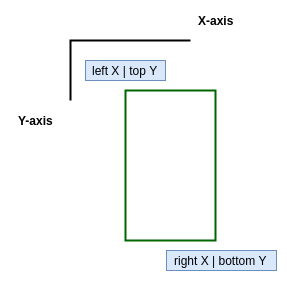
\includegraphics[width=0.4\textwidth]{img/chapters/resultados/datasets/bbox-oidv4.png}
\caption{\label{fig:bbox-oidv4}Estructura de las etiquetas de Open Images Dataset v4 \cite{OIDv4_ToolKit}}
\end{figure}

Las etiquetas que se obtienen mediante esta herramienta no tienen el formato deseado. Las etiquetas en Darknet tienen la siguiente estructura \{\texttt{label\_ID, x\_center\_norm, y\_center\_norm, width\_norm, height\_norm}\}

donde:

\begin{itemize}
    \item \textbf{label\_ID}: es un número de índice del fichero \texttt{coco.names}, empezando por el 0 y seguido de números enteros crecientes.
    \item \textbf{x\_center\_norm} = x\_center\_abs/image\_width.
    \item \textbf{y\_center\_norm} = y\_center\_abs/image\_height.
    \item \textbf{x\_center\_norm} = width\_of\_the\_label\_abs/image\_width.
    \item \textbf{x\_center\_norm} = height\_of\_the\_label\_abs/image\_height.
\end{itemize}

Es preciso señalar que todos los atributos de posición de las etiquetas de Darknet no son absolutos, sino normalizados.

Afortunadamente, el repositorio \cite{OIDv4_ToolKit} dispone del script \texttt{convert\_annotations.py} para convertir el etiquetado tanto de las imágenes de entrenamiento como las de validación del dataset \gls{oidv4} a Darknet. Antes de su ejecución, se han sustituido en el fichero \texttt{classes.txt}, situado en la raíz del repositorio, las clases que habían por defecto por el nombre de las clases que se han descargado las imágenes, en el mismo orden que cuando se nombraron en el código \ref{lst:download-oidv4_2} para que la conversión se realice correctamente. Después se puede ejecutar la siguiente línea de código:

\vspace{0.5cm}
\begin{lstlisting}[language=iPython,caption=Descarga dataset Open Images Dataset v4 (3),captionpos=b,label={lst:download-oidv4_3}]
# Convertir etiquetas al formato de Darknet
python convert_annotations.py
\end{lstlisting}

Al finalizar la conversión de las etiquetas, se han borrado las carpetas \texttt{Label} que contienen el etiquetado en el formato original. Las carpetas \texttt{obj} y \texttt{test} se han copiado a la carpeta \texttt{./data} del repositorio de \gls{yolov4} con Darknet, ya que se realizará el entrenamiento del modelo \gls{yolov4} en base al dataset personalizado en ese repositorio \cite{yolov4-darknet-github}.

\subsection{Configuración de ficheros para el entrenamiento}
\label{subsec:configuracion-ficheros-training}

Antes de comenzar el entrenamiento de la red con el dataset \gls{oidv4} es necesario configurar el fichero \texttt{.cfg} donde se encuentran las variables de la \gls{cnn} de \gls{yolov4}.

Se ha generado el fichero \texttt{yolov4-obj.cfg} basado en \texttt{yolov4.cfg}, y se han modificado los siguientes parámetros en base a las recomendaciones indicadas en \cite{yolov4-darknet-github} para el entrenamiento:

\begin{itemize}
    \item \texttt{batch} = \textbf{64} (Cantidad de imágenes y etiquetas que se calculan de una pasada en el cálculo del gradiente y se actualiza los pesos a través del \textit{backpropagation}).
    \item \texttt{subdivisions} = \textbf{16} (Cantidad de \texttt{batches} que se subdividen en cada bloque. Las imágenes de cada bloque se ejecutan en paralelo en la \gls{gpu}).
    \item \texttt{width} = \textbf{416} (Ancho del tamaño de la red. Cada imagen se redimensiona al tamaño de la red durante el entrenamiento y la detección).
    \item \texttt{height} = \textbf{416} (Altura del tamaño de la red. Cada imagen se redimensiona al tamaño de la red durante el entrenamiento y la detección).
    \item \texttt{max\_batches} = (\# de clases) * 2.000 = 4 * 2.000 = \textbf{8.000} (Número máximo de \texttt{batches}).
    \item \texttt{steps} = \textbf{6.400} (80\% de max\_batches), \textbf{7.200} (90\% de max\_batches) (Ajuste del \texttt{learning rate} después de un determinado número de \texttt{batches}).
    \item \texttt{filters} = (\# de clases + 5) * 3 = (4 + 5) * 3 = \textbf{27} (Número de núcleos convolucionales que contiene cada capa).
\end{itemize}

Se ha creado el fichero \texttt{obj.data} basado en el \texttt{coco.data} que se vio en la sección \ref{sec:evaluate-cocodataset}. En este caso, se ha especificado que el número de clases que se va a entrenar es de 4, la ubicación de los ficheros \texttt{train.txt}, \texttt{test.txt}, \texttt{coco.names} y la carpeta donde se generarán los ficheros \texttt{.weights} con los pesos de la red entrenada cada 1.000 iteraciones.

\vspace{0.5cm}
\begin{lstlisting}[language=iPython,caption=Fichero obj.data,captionpos=b,label={lst:obj-data-file}]
classes = 4
train = data/train.txt
valid = data/test.txt
names = data/obj.names
backup = /mydrive/yolov4/backup
\end{lstlisting}

Otro fichero generado ha sido el \texttt{obj.names}, basado en el \texttt{coco.names} que trae por defecto \gls{yolov4}. En este fichero se han sustituido las 80 clases de \gls{coco} que vienen predeterminadas por las 4 clases que se desean entrenar. El orden de escritura ha sido el mismo que el fichero \texttt{classes.txt}. Como ya se explicó en la sección \ref{subsec:recopilacion-etiquetado-custom-dataset}, el primer parámetro de las etiquetas de las imágenes de entrenamiento y validación es el ID de cada clase, por lo que debe de corresponder a la misma que se escribe en este fichero.

\vspace{0.5cm}
\begin{lstlisting}[language=iPython,caption=Fichero obj.names,captionpos=b,label={lst:obj-names-file}]
Person
Handbag
Backpack
Suitcase
\end{lstlisting}

Los últimos archivos de configuración necesarios antes de comenzar el entrenamiento son los ficheros \texttt{train.txt} y \texttt{test.txt}, los cuales contienen las rutas relativas a todas las imágenes de entrenamiento e imágenes de validación.

Ejecutando el siguiente script en Python se genera el fichero \texttt{train.txt}.

\vspace{0.5cm}
\begin{lstlisting}[language=iPython,caption=Generación del fichero train.txt,captionpos=b,label={lst:train-generate}]
import os

image_files = []
os.chdir(os.path.join("data", "obj"))
for filename in os.listdir(os.getcwd()):
    if filename.endswith(".jpg"):
        image_files.append("data/obj/" + filename)
os.chdir("..")
with open("train.txt", "w") as outfile:
    for image in image_files:
        outfile.write(image)
        outfile.write("\n")
    outfile.close()
os.chdir("..")
\end{lstlisting}

Para generar el fichero \texttt{test.txt}:

\vspace{0.5cm}
\begin{lstlisting}[language=iPython,caption=Generación del fichero test.txt,captionpos=b,label={lst:test-generate}]
import os

image_files = []
os.chdir(os.path.join("data", "test"))
for filename in os.listdir(os.getcwd()):
    if filename.endswith(".jpg"):
        image_files.append("data/test/" + filename)
os.chdir("..")
with open("test.txt", "w") as outfile:
    for image in image_files:
        outfile.write(image)
        outfile.write("\n")
    outfile.close()
os.chdir("..")
\end{lstlisting}

\subsection{Entrenamiento del dataset personalizado}
\label{subsec:training-custom-dataset}

Se han descargado los pesos de las capas convolucionales del modelo preentrenado \texttt{yolov4.conv.137}. El uso de estos peso hace que el detector de objetos personalizado ayuda a que converja, a que sea mucho más preciso y que no tenga que entrenar tanto tiempo.

Como último paso, se ha ejecutado el comando para realizar el entrenamiento del detector de objetos personalizado con \gls{yolov4}. Dado que se ha utilizado un conjunto de imágenes para la validación, se ha utilizado el flag \texttt{-map} para que se genere un diagrama con el \gls{map} con la finalidad de poder visualizar la precisión del modelo entrenado.

\vspace{0.5cm}
\begin{lstlisting}[language=iPython,caption=Entrenamiento del dataset personalizado,captionpos=b,label={lst:training-custom-dataset}]
# Descarga de los pesos de las capas convolucionales de YOLOv4
wget https://github.com/AlexeyAB/darknet/releases/download/darknet_yolo_v3_optimal/yolov4.conv.137

# Comenzar a entrenar la red neuronal del dataset personalizado de OIDv4
./darknet detector train data/obj.data cfg/yolov4-obj.cfg yolov4.conv.137 -dont_show -map
\end{lstlisting}

Durante el entrenamiento se puede visualizar por terminal información muy relevante como la que se muestra en la figura \ref{fig:metrics-during-train}.

\begin{figure}[ht]
\centering
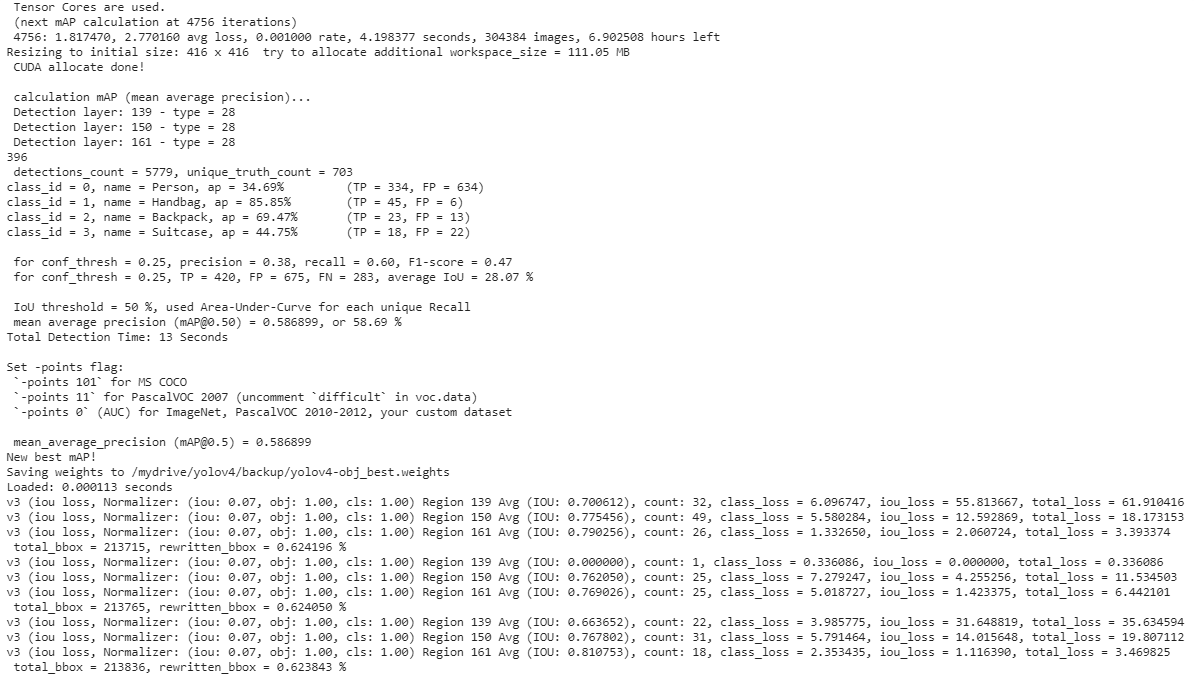
\includegraphics[width=0.9\textwidth]{img/chapters/desarrollo/metrics-during-training.png}
\caption{\label{fig:metrics-during-train}Métricas durante el entrenamiento de la red neuronal con el dataset de OIDv4}
\end{figure}

Cada cierto número de iteraciones se calcula el \gls{map} y otras métricas de interés. Siguiendo las recomendaciones de \cite{yolov4-darknet-github}, las iteraciones mínimas por cada clase para realizar un entrenamiento es de 2.000. En el primer entrenamiento del dataset personalizado se han realizado 8.000 iteraciones para 4 clases. En el caso de que se hubiera fijado unas máxima iteraciones superiores a las mínimas recomendadas, un indicio para saber que se debe finalizar el entrenamiento es cuando la media de las pérdidas (\textit{average loss}) no disminuye en las siguientes iteraciones. También, se debe de tener en cuenta que, en datasets con una dificultad alta, como es este caso, la media de pérdidas final suele ser de $\text{avg loss = 3.0}$.

Al finalizar el entrenamiento se han evaluado las métricas de calidad. Gracias al framework Darknet \cite{darknet13} es fácil poder evaluarlas aplicando el siguiente comando en el terminal:

\vspace{0.5cm}
\begin{lstlisting}[language=iPython,caption=Evaluación métricas de calidad del dataset utilizado para el entrenamiento de la red neuronal de detección de objetos,captionpos=b,label={lst:darknet-map}]
# Evaluacion de metricas de interes
./darknet detector train data/obj.data cfg/yolov4-obj.cfg /mydrive/yolov4/backup/yolov4-obj_last.weights -dont_show
\end{lstlisting}

Durante el entrenamiento se ha generado un diagrama que se encuentra en la carpeta raíz del repositorio con nombre \texttt{chart.png}, donde se puede observar la evolución de las pérdidas por el error en función de las iteraciones. En la figura \ref{fig:chart-train} se visualiza en color azul la evolución de las pérdidas y en rojo la evolución del \gls{map}.

\begin{figure}[ht]
\centering
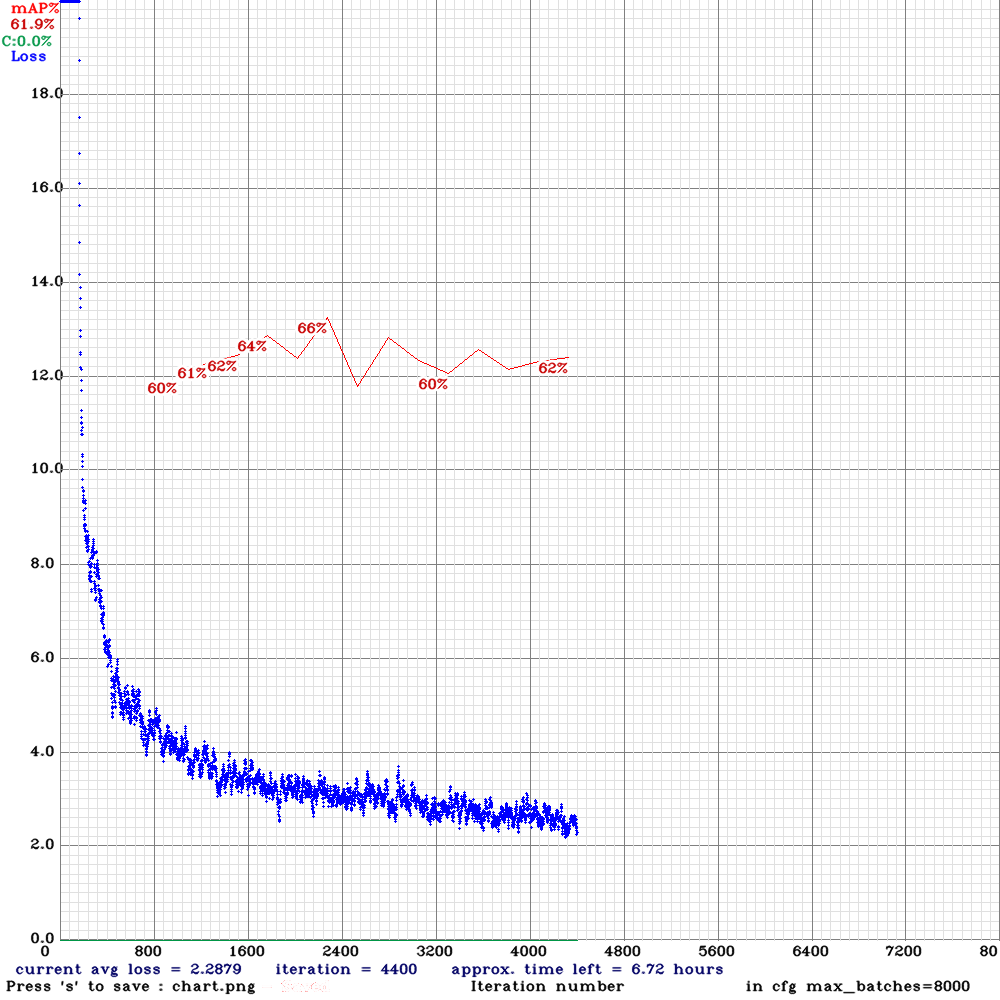
\includegraphics[width=0.5\textwidth]{img/chapters/desarrollo/chart_train.png}
\caption{\label{fig:chart-train}Evolución del mAP y pérdidas a lo largo de las interacciones durante el entrenamiento de la red neuronal con el dataset de OIDv4}
\end{figure}

Cabe resaltar que, cada 1.000 iteraciones se genera un fichero \texttt{.weights} con los pesos del modelo que estamos entrenando en \gls{yolov4} y se almacenan en la carpeta \texttt{./backup}. Es importante tener en cuenta que se ha establecido las máximas iteraciones del entrenamiento a 8.000, sin embargo, es posible que el mejores resultados en las métricas hayan sido en la iteración 5.000. Esto puede ser producido por el \textit{overfitting}. Afortunadamente, durante el entrenamiento se genera un fichero llamado \texttt{yolov4-obj\_best.weights} donde se almacenan los pesos de la red entrenada con mejores resultados. Por tanto, se ha podido ahorrar tiempo en analizar las métricas cada 1.000 iteraciones para determinar en que iteración el error era mínimo.

En la sección \ref{subsec:metricas-calidad-openimagesv4} se observarán y analizarán los resultados tanto de este entrenamiento como de un segundo que ha sido necesario ya que no se obtuvieron métricas de calidad superiores a las del dataset \gls{coco}.

\section{Seguimiento de personas y objetos con YOLOv4 y Deep SORT}
\label{sec:desarrollo-yolov4+deepsort}

En esta sección se expone el esqueleto sobre el se ha desarrollado el algoritmo de detección de objetos abandonados. Para su aplicación, se ha utilizado el algoritmo de seguimiento \gls{deepsort} trabajando conjuntamente con el detector de objetos \gls{yolov4}. La implementación que se va a exponer a continuación está totalmente inspirada en \cite{yolov4-deepsort-original}.

Se ha clonado el repositorio de GitHub de seguimiento de objetos y personas con \gls{deepsort} y \gls{yolov4} en Tensorflow \cite{yolov4-deepsort}, donde previamente se ha realizado un \textit{fork} de \cite{yolov4-deepsort-original}. Se ha empleado el entorno virtual Anaconda \texttt{yolov4-gpu} utilizado en el código \ref{lst:evaluate-yolov4-tf1}, ya que se van a utilizar las mismas versiones de librerías que en la implementación del detector de objetos con \gls{yolov4} en Tensorflow \cite{yolov4-tf-github}. Se han descargado los pesos de \gls{yolov4} previamente entrenados sobre el dataset \gls{coco} para ser convertidos a modelos Tensorflow. Una vez descargado el repositorio \cite{yolov4-deepsort}, se han creado varias ramas git para el desarrollo del proyecto. En esta parte del proyecto se va a trabajar sobre la rama \texttt{develop} para la implementación del algoritmo de seguimiento de objetos y personas con \gls{deepsort} y \gls{yolov4}.

Del mismo modo que en la sección \ref{sec:desarrollo-yolov4}, se ha utilizado en las últimas evaluaciones del algoritmo la \gls{gpu} NVIDIA Tesla T4 del servicio cloud de Google Colab, ya que se trata de la \gls{gpu} con mejores prestaciones que se puede utilizar de forma gratuita en el servicio de Google. Proporciona la mayor velocidad de \gls{fps} en las evaluaciones de los algoritmos.

\vspace{0.5cm}
\begin{lstlisting}[language=iPython,caption=Evaluación del seguimiento de objetos Deep SORT y YOLOv4 en Tensorflow (1),captionpos=b,label={lst:evaluate-deepsort-tf1}]
# Descarga del repositorio de GitHub
git clone https://github.com/jmudy/yolov4-deepsort

# Entrar dentro de la carpeta del repositorio
cd yolov4-deepsort

# Cambiar a la rama de git develop y comprobar que nos encontramos en ella
git checkout develop
git branch -a

# Descarga de los pesos de YOLOv4
wget https://github.com/AlexeyAB/darknet/releases/download/darknet_yolo_v3_optimal/yolov4.weights -P ./data/
\end{lstlisting}

En el código \ref{lst:evaluate-deepsort-tf2} se muestra el comando para convertir el modelo preentrenado de \gls{yolov4} en Darknet a Tensorflow. Se ha especificado un tamaño de 608x608, por dos motivos. El primero, es el mismo tamaño de redimensionamiento de las imágenes de entrada de la capa de la red Darknet, con lo cual, se puede comparar ambos modelos en las mismas condiciones en la etapa de detección. Segundo, se han obtenido mejores resultados que empleando el clásico tamaño de 416x416.

\vspace{0.5cm}
\begin{lstlisting}[language=iPython,caption=Evaluación del seguimiento de objetos Deep SORT y YOLOv4 en Tensorflow (2),captionpos=b,label={lst:evaluate-deepsort-tf2}]
# Convertir pesos de YOLOv4 Darknet a Tensorflow
python save_model.py --weights ./data/yolov4.weights --output ./checkpoints/yolov4-608 --input_size 608 --model yolov4
\end{lstlisting}

En el código \ref{lst:evaluate-deepsort-tf3} se puede observar el comando que se ha utilizado para la ejecución del algoritmo de seguimiento de \gls{deepsort} con \gls{yolov4} en Tensorflow. Como se puede apreciar en las primeras líneas del script \texttt{object\_tracker.py} \cite{yolov4-deepsort}, se disponen de una serie de flags donde se pueden indicar una gran variedad de parámetros, del mismo modo que en \cite{yolov4-tf-github-original}. En este caso, se ha indicado que se quiere utilizar un modelo de \gls{yolov4} convertido a Tensorflow con tamaño de redimensionamiento 608x608 (si no se indica, el código por defecto busca un modelo de tamaño 416x416). Se ha especificado que se quiere emplear en la etapa de detección \gls{yolov4}, ya que este repositorio también permite ejecutar la detección de objetos sobre \gls{yolo}v3. También se han incluido los flags \texttt{-{}-count} para obtener por terminal el número de objetos que se están rastreando y \texttt{-{}-info} para obtener por terminal las variables \texttt{track.track\_id} que indica la identidad del objeto rastreado en cada fotograma, \texttt{class\_name} que indica el nombre de la clase y \{\texttt{bbox[0], bbox[1], bbox[2], bbox[3]}\} para conocer los valores de \{xmin, ymin, xmax, ymax\} de los cuadros delimitadores.

\vspace{0.5cm}
\begin{lstlisting}[language=iPython,caption=Evaluación del seguimiento de objetos Deep SORT y YOLOv4 en Tensorflow (3),captionpos=b,label={lst:evaluate-deepsort-tf3}]
# Ejecutar algoritmo de seguimiento de objetos con Deep SORT y YOLOv4 en Tensorflow
!python object_tracker.py --video {input_file_name.mp4} --output {output_file_name.avi} --model yolov4 --size 608 --weights ./checkpoints/yolov4-608 --count --info
\end{lstlisting}

En la figura \ref{fig:prueba-deepsort-frame53} se muestra un fotograma del seguimiento de objetos y personas en una secuencia extraída de \cite{Benfold2011StableMT}, un dataset que no se va a contemplar en este proyecto, pero que se utiliza con mucha frecuencia en la evaluación de algoritmos de detección y seguimiento de objetos. Como se puede apreciar, cada persona y objeto detectado tiene una identidad única asignada durante el rastreo. Como se pudo ver en la figura \ref{fig:mot-gba}, en los \gls{mot}, hay una primera etapa correspondiente a la detección (representado con el cuadro delimitador en color blanco) y una segunda etapa correspondiente al seguimiento (representado con los cuadros delimitadores de color azul y naranja). En esta propuesta únicamente se va a visualizar el cuadro delimitador que corresponde al seguimiento, asignando un color a cada elemento detectado. Cabe destacar que, en los primeros fotogramas de la secuencia se identificó como una motocicleta la bicicleta que acompaña a la persona con ID \texttt{person-21}. Durante los fotogramas siguientes se mantiene ese seguimiento erróneo. Se trata de un error poco frecuente que sucede hasta que se pierde el rastreo del objeto y se vuelva a asignar una nueva identidad después de la detección.

\begin{figure}[ht]
\centering
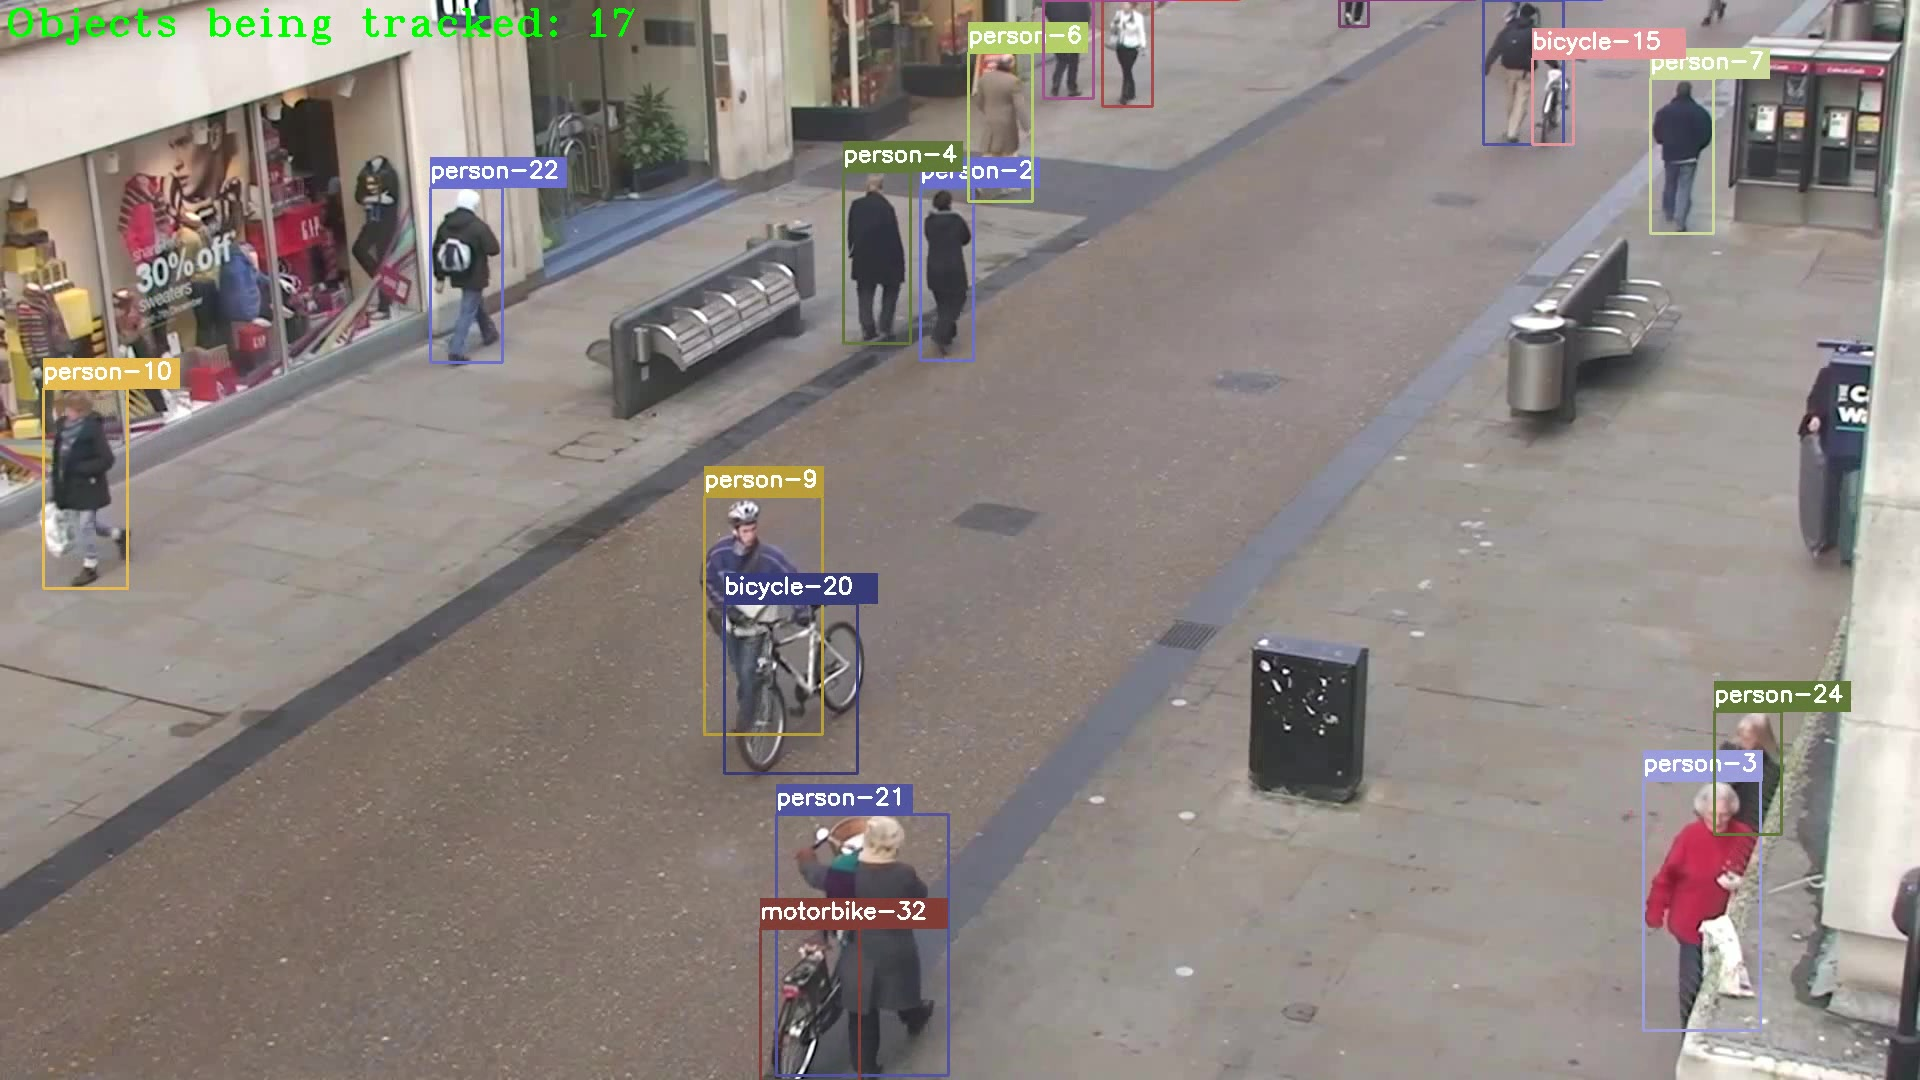
\includegraphics[width=0.45\textwidth]{img/chapters/desarrollo/prueba-deepsort-frame53.jpg}
\caption{\label{fig:prueba-deepsort-frame53}Ejemplo de MOT con Deep SORT en \cite{Benfold2011StableMT}}
\end{figure}

En el siguiente código \ref{lst:deepsort-original-test1}, se muestra la información que se arroja por terminal al ejecutar el script \texttt{object\_tracker.py} con los flags \texttt{-{}-count} y \texttt{-{}-info}. Por cada fotograma del vídeo procesado se muestra la cantidad de objetos que se están rastreando, el ID de cada persona u objeto detectado y el valor de las variables que componen los cuadros delimitadores. También, se indica la velocidad a la que se ha procesado el vídeo sobre una \gls{gpu} NVIDIA Tesla T4. El acceso a las variables de ID y parámetros de los cuadros delimitadores en cada fotograma facilitarán el desarrollo del algoritmo de detección de objetos abandonados en la sección \ref{sec:algoritmo-object-detection}.

\vspace{0.5cm}
\begin{lstlisting}[language=iPython,caption=Prueba test del seguimiento de objetos Deep SORT y YOLOv4,captionpos=b,label={lst:deepsort-original-test1}]
Frame number:  53
Objects being tracked: 17
Tracker ID:  1, Class: person,    BBox Coords (xmin,ymin,xmax,ymax): (1483,0,1563,144)
Tracker ID:  2, Class: person,    BBox Coords (xmin,ymin,xmax,ymax): (920,187,973,360)
Tracker ID:  3, Class: person,    BBox Coords (xmin,ymin,xmax,ymax): (1643,780,1760,1030)
Tracker ID:  4, Class: person,    BBox Coords (xmin,ymin,xmax,ymax): (843,171,910,343)
Tracker ID:  6, Class: person,    BBox Coords (xmin,ymin,xmax,ymax): (968,52,1032,201)
Tracker ID:  7, Class: person,    BBox Coords (xmin,ymin,xmax,ymax): (1650,78,1713,233)
Tracker ID:  9, Class: person,    BBox Coords (xmin,ymin,xmax,ymax): (704,496,822,734)
Tracker ID: 10, Class: person,    BBox Coords (xmin,ymin,xmax,ymax): (43,388,127,588)
Tracker ID: 13, Class: person,    BBox Coords (xmin,ymin,xmax,ymax): (1102,0,1152,106)
Tracker ID: 15, Class: bicycle,   BBox Coords (xmin,ymin,xmax,ymax): (1532,58,1573,144)
Tracker ID: 16, Class: person,    BBox Coords (xmin,ymin,xmax,ymax): (1339,0,1368,26)
Tracker ID: 17, Class: person,    BBox Coords (xmin,ymin,xmax,ymax): (1043,0,1093,98)
Tracker ID: 20, Class: bicycle,   BBox Coords (xmin,ymin,xmax,ymax): (724,603,857,773)
Tracker ID: 21, Class: person,    BBox Coords (xmin,ymin,xmax,ymax): (776,814,948,1075)
Tracker ID: 22, Class: person,    BBox Coords (xmin,ymin,xmax,ymax): (430,187,502,362)
Tracker ID: 24, Class: person,    BBox Coords (xmin,ymin,xmax,ymax): (1714,711,1781,834)
Tracker ID: 32, Class: motorbike, BBox Coords (xmin,ymin,xmax,ymax): (760,928,859,1080)
FPS: 10.06
\end{lstlisting}

Como se puede apreciar en la figura \ref{fig:prueba-deepsort-frame53} y el código \ref{lst:deepsort-original-test1} se están rastreando clases que no son de interés para el objetivo de este \gls{tfm}, en concreto, se identifica las 80 clases que componen el dataset \gls{coco} y que se pueden ver dentro del fichero \texttt{data/classes/coco.names}. Así pues, se va a filtrar las detecciones para que solo se muestre por pantalla el seguimiento de las clases: \texttt{person, backpack, handbag} y \texttt{suitcase}. Sin embargo, se pueden modificar fácilmente unas pocas líneas de código para rastrear las clases que son de interés.

Para filtrar las clases de interés solo ha sido necesario comentar la línea 136 y descomentar la línea 137 del script \texttt{object\_tracker.py} \cite{yolov4-deepsort} añadiendo las clases \texttt{person, backpack, handbag} y \texttt{suitcase}. Dentro de la lista \texttt{allowed\_classes} simplemente se han añadido las clases que se desea rastrear. En el siguiente código \ref{lst:allowed_classes} se muestran los cambios realizados en las líneas de código nombradas.

\vspace{0.5cm}
\begin{lstlisting}[language=iPython,caption=Clases permitidas en el seguimiento de objetos con Deep SORT,captionpos=b,label={lst:allowed_classes}]
    # by default allow all classes in .names file
    #allowed_classes = list(class_names.values())
    allowed_classes = ['person', 'handbag', 'backpack', 'suitcase']
\end{lstlisting}

Como se ha podido observar en la figura \ref{fig:prueba-deepsort-frame53} cada objeto o persona rastreada se representa con un cuadro delimitador de distinto color. Para evitar la dificultad de visualizar con claridad se ha cambiado verde la clase \texttt{person} y a color azul las clases \texttt{backpack, handbag y suitcase}. Para ello, se han modificado las líneas 190-201 tal y como se puede ver en el código \ref{lst:colors-allowed_classes}.

\vspace{0.5cm}
\begin{lstlisting}[language=iPython,caption=Colores y cuadros delimitadores de las clases en el seguimiento,captionpos=b,label={lst:colors-allowed_classes}]
        # draw bbox on screen only person, handbag, backpack and suitcase
        color1 = (50, 203, 115)
        color2 = (50, 138, 203)

        if class_name == 'person':
            cv2.rectangle(frame, (int(bbox[0]), int(bbox[1])), (int(bbox[2]), int(bbox[3])), color1, 1)
            cv2.rectangle(frame, (int(bbox[0]), int(bbox[1]-20)), (int(bbox[0])+(len(class_name)+len(str(track.track_id)))*12, int(bbox[1])), color1, -1)
            cv2.putText(frame, class_name + "-" + str(track.track_id),(int(bbox[0]), int(bbox[1]-5)), cv2.FONT_HERSHEY_SIMPLEX, 0.50, (255,255,255), 1, cv2.LINE_AA)

        elif class_name == 'handbag' or 'backpack' or 'suitcase':
            cv2.rectangle(frame, (int(bbox[0]), int(bbox[1])), (int(bbox[2]), int(bbox[3])), color2, 1)
            cv2.rectangle(frame, (int(bbox[0]), int(bbox[1]-20)), (int(bbox[0])+(len(class_name)+len(str(track.track_id)))*12, int(bbox[1])), color2, -1)
            cv2.putText(frame, class_name + "-" + str(track.track_id),(int(bbox[0]), int(bbox[1]-5)), cv2.FONT_HERSHEY_SIMPLEX, 0.50, (255,255,255), 1, cv2.LINE_AA)
\end{lstlisting}

En la siguiente figura \ref{fig:prueba2-deepsort-frame439} se refleja el resultado de filtrar las clases y utilizar únicamente dos colores para los cuadros delimitadores para cada una de las clases de objetos que se desea rastrear. De esta manera resulta más sencillo trabajar con los objetos de interés de cara al desarrollo del algoritmo de detección de objetos abandonados en la siguiente sección \ref{sec:algoritmo-object-detection}.

\begin{figure}[ht]
\centering
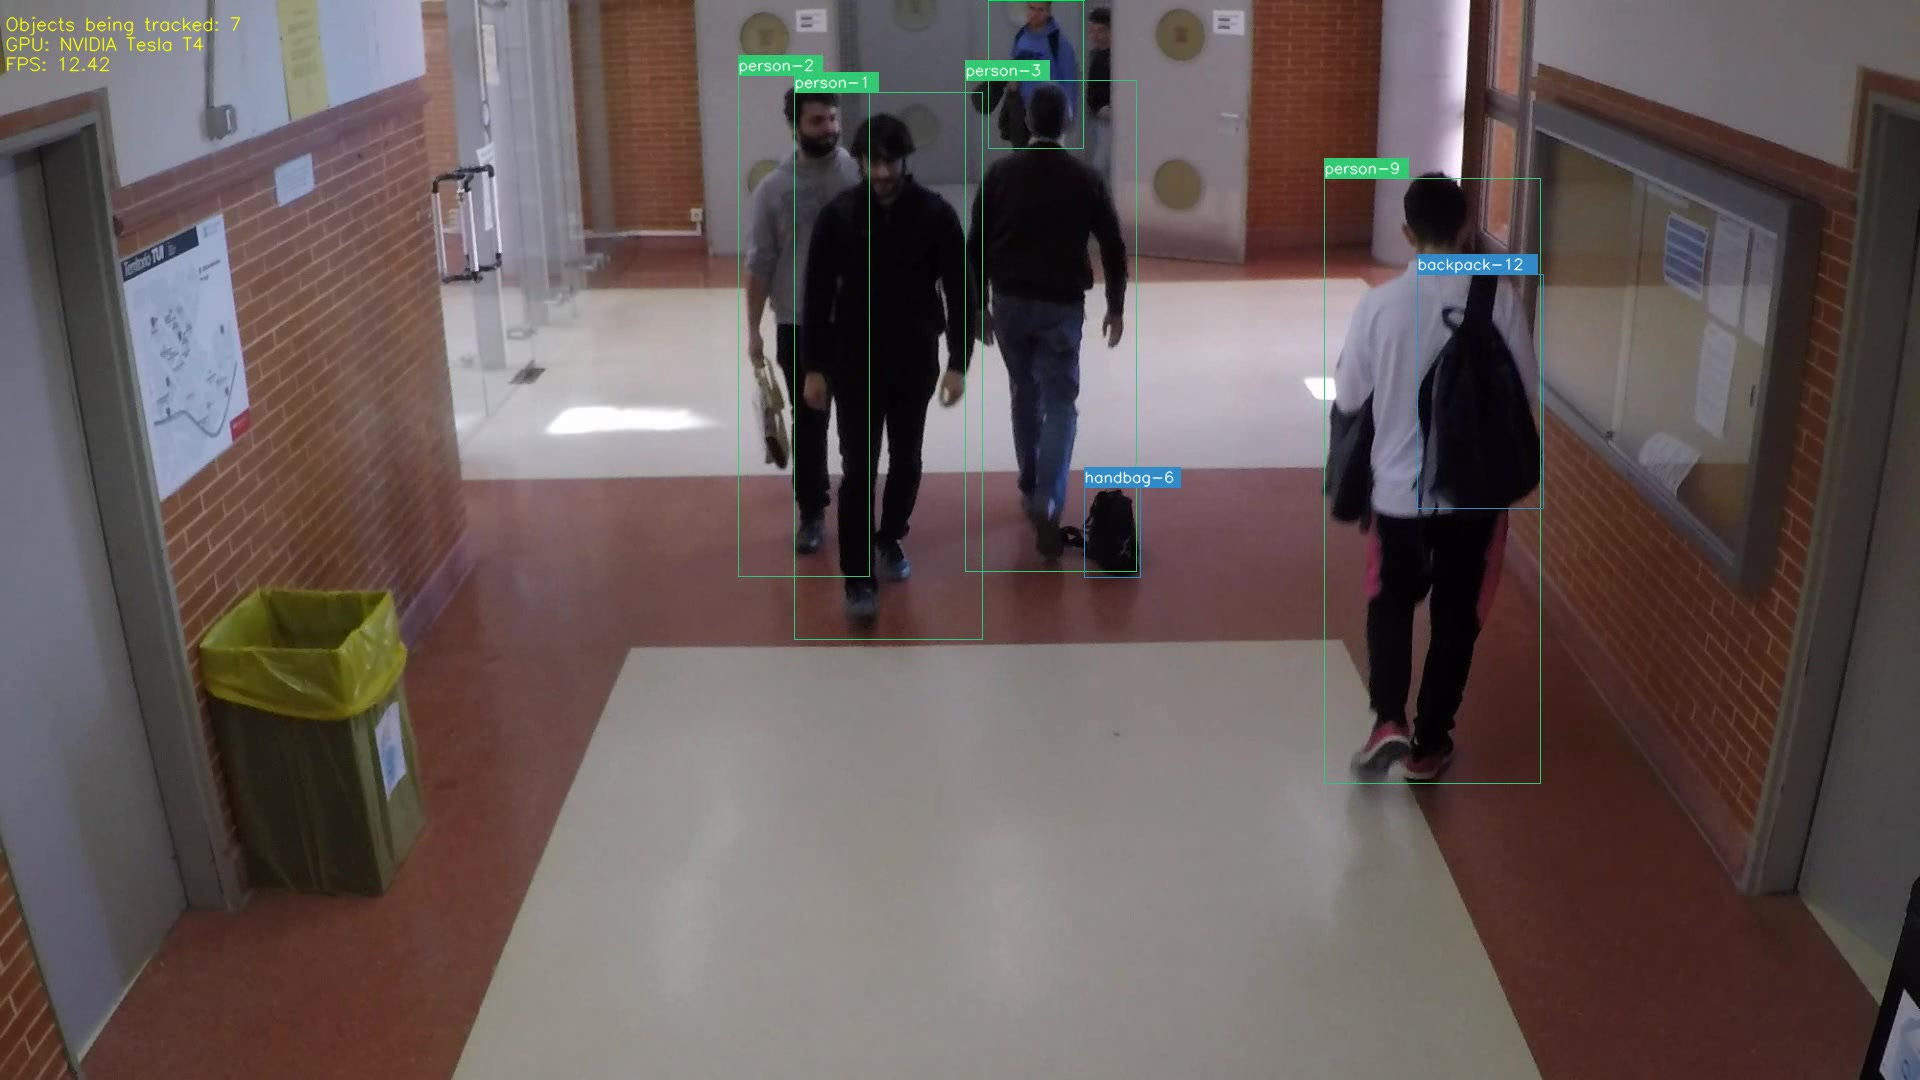
\includegraphics[width=0.45\textwidth]{img/chapters/desarrollo/prueba2-deepsort-frame439.jpg}
\caption{\label{fig:prueba2-deepsort-frame439}Ejemplo de MOT con Deep SORT filtrando clases de interés en \cite{gba-dataset}}
\end{figure}

Las últimas evaluaciones del algoritmo de seguimiento se han realizado con Google Colab. En el siguiente \href{https://colab.research.google.com/drive/18vL9LH8e9VaimA9LzBD35Cn4AOm6C17I?usp=sharing}{link} se puede ejecutar el Notebook donde se realizan los mismos pasos descritos anteriormente. Todos los resultados obtenidos durante la evaluación del seguimiento de objetos y personas con \gls{deepsort} y \gls{yolov4} en Tensorflow se visualizarán y analizarán en la sección \ref{subsec:resultados-yolov4+deepsort}.

\section{Algoritmo de detección de objetos abandonados}
\label{sec:algoritmo-object-detection}

En esta sección se explica en detalle la propuesta de algoritmo para la detección de objetos abandonados a partir del algoritmo de detección \gls{yolov4} junto con el algoritmo de seguimiento \gls{deepsort}.

Durante los primeros 5 segundos de ejecución de script el algoritmo calcula la distancia entre las personas y los objetos de interés mediante la función \texttt{asociar}. Si el vídeo de entrada tiene un frame rate de 30, el script estará calculando la distancia entre los centroides de los cuadros delimitadores durante las primeras 150 iteraciones del bucle while del programa principal.

La función \texttt{asociar} devuelve tres valores. Los dos primeros son el número identificador de la persona y del objeto que le ha sido asociado mediante el algoritmo de seguimiento, y el último valor es el de la distancia. Dado que en un fotograma cualquiera se pueden encontrar numerosas personas y objetos de interés, el script actualiza la asociación persona-objeto comparando la distancia medida con la calculada en el fotograma anterior y quedándose con la más pequeña, de tal manera que se garantiza que dicho objeto es propiedad de la persona a la que se le ha asignado.

El siguiente código \ref{lst:diccionario-centroides} muestra la estructura del diccionario \texttt{centroid\_dict}. Está formado por diferentes elementos de los cuales el primero es el número identificador del objeto o persona detectado y los dos siguientes son las coordenadas $x,y$ de los centroides de los cuadros delimitadores.

\vspace{0.5cm}
\begin{lstlisting}[language=iPython,caption=Diccionario centroides personas y objetos,captionpos=b,label={lst:diccionario-centroides}]
centroid_dict = idx, (int(x), int(y), xmin, ymin, xmax, ymax)
\end{lstlisting}

La función \texttt{is\_close} calcula la distancia euclideana en píxeles de los centroides de los objetos detectados. Posteriormente, mediante un bucle for y la función \texttt{combinations} de la librería \texttt{itertools} se calcula la distancia entre todos los objetos y personas detectables en un determinado fotograma.

\vspace{0.5cm}
\begin{lstlisting}[language=iPython,caption=Cálculo distancia entre persona y objetos,captionpos=b,label={lst:calculo-distancia-persona-objeto}]
def is_close(p1, p2):

    dst = math.sqrt(p1**2 + p2**2)
    
    return dst 

for (id1, p1), (id2, p2) in combinations(centroid_dict.items(), 2):
    dx, dy = p1[0] - p2[0], p1[1] - p2[1]
    distance = is_close(dx, dy)
\end{lstlisting}

En el caso de que el identificador del primer elemento corresponda a la clase persona y el segundo a la clase de un objeto de interés se guardarán los datos en una matriz con nombre \texttt{distances}. Esta matriz está formada por 3 columnas, donde se alojan el número de identidad de la persona y objeto que sí que cumplen con la condición de asociación y la distancia, y tantas filas como personas se detecten durante el paso de los fotogramas. Como se acaba de comentar anteriormente, al guardar los datos en esta matriz se tendrá en cuenta que la distancia entre la persona y el objeto sea la mínima calculada durante los primeros 5 segundos de vídeo.

Tal y como se puede contemplar en la figura \ref{fig:abandoned-object-scheme}, en el caso de que un objeto de interés no se encontrase durante los primeros 5 segundos de la secuencia de vídeo a una distancia máxima de 2 veces el ancho del cuadro delimitador de una persona, se considera que el objeto no tiene propietario, y por tanto no se encontrará dentro de la matriz \texttt{distances}. En ese caso aparecerá un mensaje de objeto abandonado cuando transcurran 15 segundos estando el objeto estático dentro del plano.

En el caso de que sí que exista asociación, es decir, que un objeto se encuentre a una distancia máxima en píxeles del doble del ancho del cuadro delimitador de una persona, y además, sea la distancia mínima de entre todos los objetos que se ha calculado su distancia hasta el sujeto, el algoritmo continuará leyendo el tercer valor de la columna del matriz \texttt{distances} para comprobar si la persona que es portadora del objeto que se le ha sido asignado abandona o no el objeto en los siguientes fotogramas.

\begin{figure}[ht]
\centering
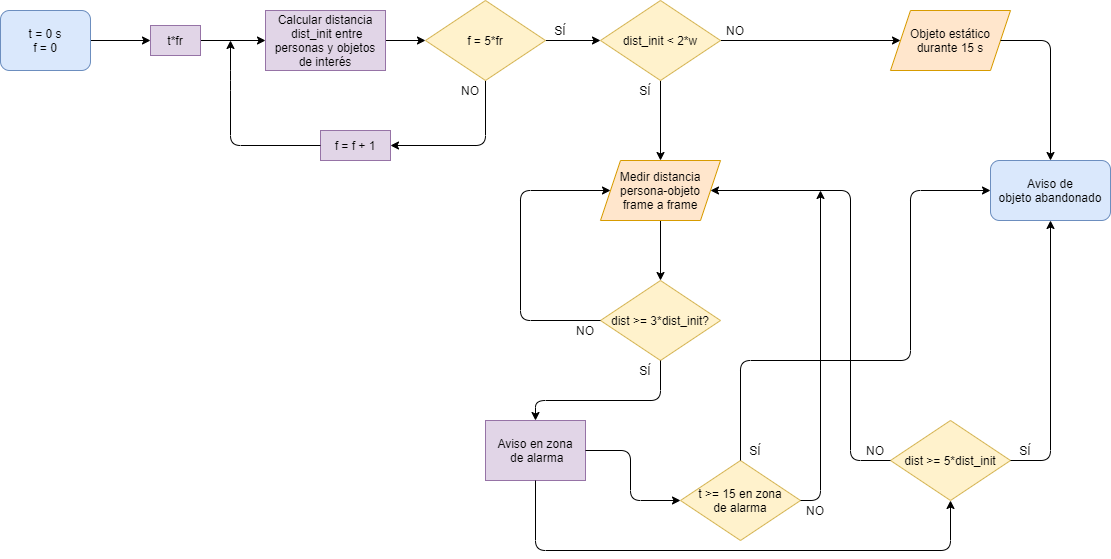
\includegraphics[width=1\textwidth]{img/chapters/desarrollo/abandoned-object-scheme.png}
\caption{\label{fig:abandoned-object-scheme}Esquema hipótesis detección objeto abandonado}
\end{figure}

En la siguiente figura \ref{fig:link-persona-objeto} se muestra como la persona con número de identidad 5 se le ha asignado como objeto de su propiedad la maleta con número de identidad 2. Al crearse la asociación persona-objeto se dibuja automáticamente una línea que une ambos centroides indicando que la asociación se ha realizado correctamente.

\begin{figure}[ht]
\centering
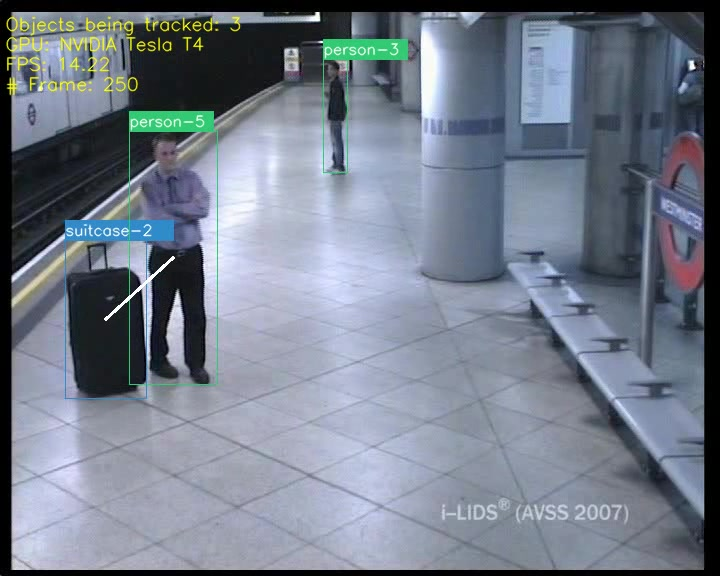
\includegraphics[width=0.4\textwidth]{img/chapters/desarrollo/link-persona-objeto.jpg}
\caption{\label{fig:link-persona-objeto}Asociación persona-objeto \cite{AVSSAB2007-dataset}}
\end{figure}

Si la distancia entre la persona y objeto es mayor o igual a 3 veces la distancia mínima que se calculó en el momento de la asociación se indicará que el objeto se encuentra en riesgo de abandono, indicando mediante un color amarillo los cuadros delimitadores de la persona y objeto así como una línea que une ambos centroides. Como se puede observar en el diagrama de funcionamiento del algoritmo en la figura \ref{fig:abandoned-object-scheme}, en el caso de que este suceso no ocurra el algoritmo continuará evaluando la distancia entre personas y objetos asociados hasta que ocurra algún incumplimiento.

\begin{figure}[ht]
\centering
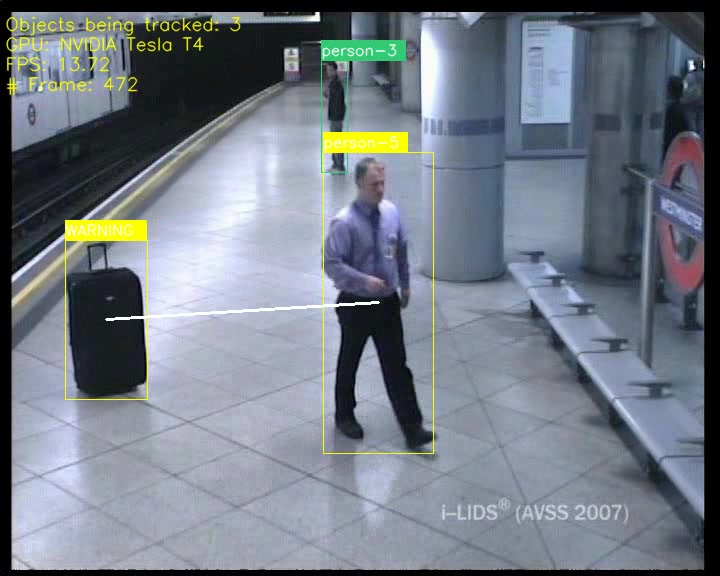
\includegraphics[width=0.4\textwidth]{img/chapters/desarrollo/warning-abandono.jpg}
\caption{\label{fig:warning-abandono}Aviso de alerta posible objeto abandonado \cite{AVSSAB2007-dataset}}
\end{figure}

En el caso de que el objeto se encuentre en zona de alarma, pueden ocurrir dos sucesos. El primero es que el objeto se encuentre de manera estática durante los siguientes 15 segundos dentro de esa zona de alarma (persona y objeto se encuentran a más de 3 veces la distancia de asociación inicial). En ese caso se considerará que el objeto ha sido abandonado. El segundo suceso es que la persona siga alejándose del objeto del que es propietario a una distancia igual o mayor a 5 veces la distancia inicial de asociación o desaparezca del plano. En esa situación el objeto se considerará abandonado.

Como se puede observar en la figura \ref{fig:abandono-objeto-avss} anterior, la persona portadora de la maleta se aleja a una distancia en píxeles mayor a 5 veces la distancia de asociación. En ese caso se indicará que el objeto ha sido abandonado con un color rojo en los cuadros delimitadores de la persona y el objeto abandonado, de manera que se podrá identificar la identidad de la persona que abandonó el objeto. De la misma forma que en el caso de cuando el objeto se encontraba en zona de alarma, se dibujará una línea que une el centroide entre la persona y el objeto para visualizar con mayor facilidad la persona y objeto asociado que está provocando un abandono.

Del mismo modo que en la sección \ref{sec:desarrollo-yolov4}, se ha utilizado en las últimas evaluaciones del algoritmo la \gls{gpu} NVIDIA Tesla T4 del servicio cloud de Google Colab, ya que se trata de la \gls{gpu} con mejores prestaciones que se puede utilizar de forma gratuita en el servicio de Google. Proporciona la mayor velocidad de \gls{fps} en las evaluaciones de los algoritmos.

\begin{figure}[ht]
\centering
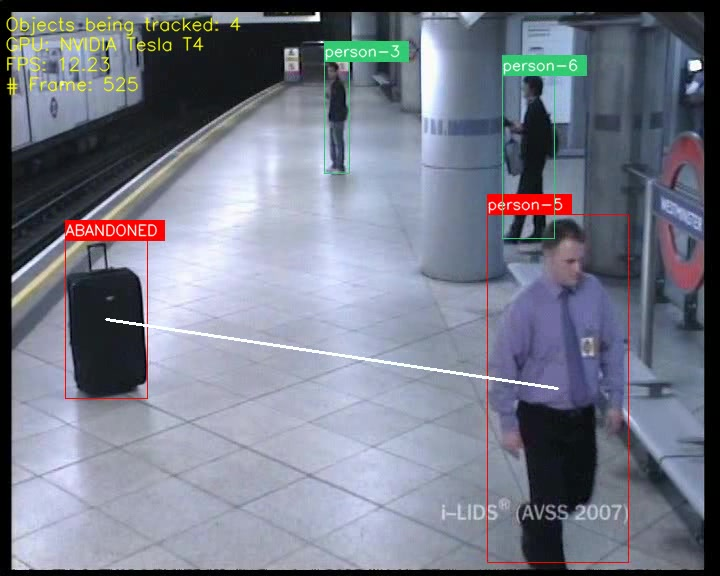
\includegraphics[width=0.4\textwidth]{img/chapters/desarrollo/abandono-objeto-avss.jpg}
\caption{\label{fig:abandono-objeto-avss}Detección de objeto abandonado \cite{AVSSAB2007-dataset}}
\end{figure}

Para ejecutar el algoritmo de detección de objetos abandonados se debe de acceder a la misma carpeta \texttt{yolov4-deepsort} que se utilizó para evaluar el funcionamiento del seguimiento de objetos con \gls{yolov4} y \gls{deepsort} en la sección \ref{sec:desarrollo-yolov4+deepsort}. En esta ocasión se deberá de cambiar de rama de Git para poder acceder a los ficheros necesarios. Dado que se trata de otra rama no se habrán guardado los cambios realizados en la rama \texttt{develop}, por tanto, ha sido necesario descargar de nuevo los pesos de \gls{yolov4} Darknet.

\vspace{0.5cm}
\begin{lstlisting}[language=iPython,caption=Evaluación de la detección de objetos abandonados con DeepSORT y YOLOv4 en Tensorflow (1),captionpos=b,label={lst:evaluate-abandoned-object1}]
# Entrar dentro de la carpeta del repositorio
cd yolov4-deepsort

# Cambiar a la rama de git abandoned y comprobar que nos encontramos en ella
git checkout abandoned
git branch -a

# Descarga de los pesos de YOLOv4
wget https://github.com/AlexeyAB/darknet/releases/download/darknet_yolo_v3_optimal/yolov4.weights -P ./data/
\end{lstlisting}

Del mismo modo que en la sección \ref{sec:desarrollo-yolov4+deepsort}, se ha convertido el modelo Darknet a Tensorflow con un tamaño de redimensionamiento de 608x608 ejecutando el comando que se muestra en el código \ref{lst:evaluate-abandoned-object2}, dado que han obtenido mejores resultados que con un tamaño de 416x416.

\vspace{0.5cm}
\begin{lstlisting}[language=iPython,caption=Evaluación de la detección de objetos abandonados con DeepSORT y YOLOv4 en Tensorflow (2),captionpos=b,label={lst:evaluate-abandoned-object2}]
# Convertir pesos de YOLOv4 Darknet a Tensorflow
python save_model.py --weights ./data/yolov4.weights --output ./checkpoints/yolov4-608 --input_size 608 --model yolov4
\end{lstlisting}

En el código \ref{lst:evaluate-abandoned-object3} se puede observar el comando que se ha utilizado para la ejecución del algoritmo de detección de objetos abandonados con \gls{deepsort} y \gls{yolov4} en Tensorflow. De igual manera al código \ref{lst:evaluate-deepsort-tf3} se ha utilizado los flags \texttt{-{}-info} y \texttt{-{}-count} para obtener los valores \{xmin, ymin, xmax, ymax\} de los cuadros delimitadores así como el número de objetos y personas que se está detectando en pantalla.

\vspace{0.5cm}
\begin{lstlisting}[language=iPython,caption=Evaluación de la detección de objetos abandonados con DeepSORT y YOLOv4 en Tensorflow (3),captionpos=b,label={lst:evaluate-abandoned-object3}]
# Ejecutar algoritmo de deteccion objetos abandonados con Deep SORT y YOLOv4 en Tensorflow
!python abandoned_object.py --video {input_file_name.mp4} --output {output_file_name.avi} --model yolov4 --size 608 --weights ./checkpoints/yolov4-608 --count --info
\end{lstlisting}

Las últimas evaluaciones del algoritmo de seguimiento se han realizado con Google Colab. En el siguiente \href{https://colab.research.google.com/drive/18vL9LH8e9VaimA9LzBD35Cn4AOm6C17I?usp=sharing}{link} se puede ejecutar el Notebook donde se realizan los mismos pasos descritos anteriormente. Todos los resultados obtenidos durante la evaluación del seguimiento de objetos y personas con \gls{deepsort} y \gls{yolov4} en Tensorflow se visualizarán y analizarán en la sección \ref{subsec:resultados-abandon-algorithm}.

\section{Conclusiones}
\label{sec:conclu-desarrollo}

Este capítulo ha tenido como objetivo el desarrollo de un algoritmo de detección de objetos abandonados utilizando \gls{yolov4} como algoritmo de detección y \gls{deepsort} como algoritmo de seguimiento de objetos y personas. \gls{yolov4} viene previamente entrenado sobre el dataset \gls{coco}. Dado que se quiere utilizar un sistema donde no se necesita detectar las 80 clases de \gls{coco} y solo se precisa la detección de personas y los objetos de interés: mochilas, maletas y bolsas de mano, se ha entrenado dos modelos de \gls{yolov4} a partir de un dataset personalizado \gls{oidv4} con la finalidad de obtener mayores valores en las métricas de calidad sobre dichas clases. Variando los parámetros de la \gls{cnn} así como el número de clases y de imágenes de entrenamiento y evaluación no se han conseguido mejorar las métricas que se obtienen con \gls{coco}. Por tanto, se ha decidido continuar el desarrollo del proyecto con el modelo preentrenado de \gls{yolov4}.

En primer lugar se ha probado \gls{yolov4} sobre el framework Darknet original. Para facilitar la programación de los scripts en la detección seguimiento y detección de objetos abandonados con Python, se ha decidido convertir el modelo \gls{yolov4} a Tensorflow, dado que Darknet no es de uso extendido y puede resultar más díficil solucionar los posibles errores que puedan aparecer.

Las implementaciones tanto de \gls{yolov4} como de \gls{deepsort} han estado totalmente inspiradas en las aplicaciones desarrolladas en los repositorios de GitHub \cite{yolov4-tf-github-original} y \cite{yolov4-deepsort-original}. Se han realizado las modificaciones oportunas para satisfacer las necesidades de cara a la etapa de desarrollo del algoritmo de detección de objetos abandonados, como es la filtración en la etapa de detección para que solo tenga en cuenta las clases de interés que se quieren detectar e ignore el resto de las clases de \gls{coco}.

Con la reciente llegada de \gls{yolov4} se ha podido aumentar la precisión en las detecciones que se realizaron con versiones previas de \gls{yolo} en \cite{valdivieso2018}. Además, la implementación de \gls{yolov4} junto con \gls{deepsort}, que incluye tanto filtros de Kalman como el algoritmo húngaro, ha provocado un mejor rastreo de los objetos y personas respecto a las propuestas que se realizaron en \cite{valdivieso2018} utilizando únicamente filtros de Kalman.

Una vez establecido como base del proyecto la utilización de \gls{yolov4} como algoritmo de detección y \gls{deepsort} como algoritmo de seguimiento de objetos y personas se ha diseñado un algoritmo de detección de objetos abandonados para aplicaciones de videovigilancia en tiempo real basado en \cite{valdivieso2018}.

Para ello, se han tenido en cuenta dos posibles escenarios. En el primero, se trata de cuando un objeto está alejado de cualquier persona y además se encuentra de manera estática durante más de 15 segundos. En ese caso se establece que el objeto ha sido previamente abandonado y además no se le puede asignar ningún propietario del mismo. En el segundo escenario se asocian los objetos a las personas más cercanas que se encuentran durante los primeros segundos de la secuencia de vídeo. Una vez establecida la asociación persona-objeto se estudia cuando la distancia que une ambos se aleja más de cierta distancia. Primeramente, se establece una distancia de zona de alarma donde el objeto es candidato a poder ser abandonado. Esta distancia es medida en píxeles entre los centroides de la persona y el objeto asociado. En el caso de que la persona se aleje más de la distancia máxima permitida o desaparezca del plano de la cámara, se lanzará un aviso por pantalla de que el objeto ha sido abandonado.

Cuando el algoritmo de seguimiento con \gls{deepsort} trabaja correctamente sin perder la identidad de las personas y objetos que se estaban detectando el algoritmo de detección de objetos abandonados funciona de forma eficiente y sin fallos. Sin embargo, tal y como se verá en la sección \ref{subsec:resultados-abandon-algorithm}, pueden aparecer fenómenos que produzcan la incapacidad de detectar un objeto abandonado.